% Options for packages loaded elsewhere
\PassOptionsToPackage{unicode}{hyperref}
\PassOptionsToPackage{hyphens}{url}
%
\documentclass[
]{book}
\usepackage{amsmath,amssymb}
\usepackage{lmodern}
\usepackage{iftex}
\ifPDFTeX
  \usepackage[T1]{fontenc}
  \usepackage[utf8]{inputenc}
  \usepackage{textcomp} % provide euro and other symbols
\else % if luatex or xetex
  \usepackage{unicode-math}
  \defaultfontfeatures{Scale=MatchLowercase}
  \defaultfontfeatures[\rmfamily]{Ligatures=TeX,Scale=1}
\fi
% Use upquote if available, for straight quotes in verbatim environments
\IfFileExists{upquote.sty}{\usepackage{upquote}}{}
\IfFileExists{microtype.sty}{% use microtype if available
  \usepackage[]{microtype}
  \UseMicrotypeSet[protrusion]{basicmath} % disable protrusion for tt fonts
}{}
\makeatletter
\@ifundefined{KOMAClassName}{% if non-KOMA class
  \IfFileExists{parskip.sty}{%
    \usepackage{parskip}
  }{% else
    \setlength{\parindent}{0pt}
    \setlength{\parskip}{6pt plus 2pt minus 1pt}}
}{% if KOMA class
  \KOMAoptions{parskip=half}}
\makeatother
\usepackage{xcolor}
\usepackage{longtable,booktabs,array}
\usepackage{calc} % for calculating minipage widths
% Correct order of tables after \paragraph or \subparagraph
\usepackage{etoolbox}
\makeatletter
\patchcmd\longtable{\par}{\if@noskipsec\mbox{}\fi\par}{}{}
\makeatother
% Allow footnotes in longtable head/foot
\IfFileExists{footnotehyper.sty}{\usepackage{footnotehyper}}{\usepackage{footnote}}
\makesavenoteenv{longtable}
\usepackage{graphicx}
\makeatletter
\def\maxwidth{\ifdim\Gin@nat@width>\linewidth\linewidth\else\Gin@nat@width\fi}
\def\maxheight{\ifdim\Gin@nat@height>\textheight\textheight\else\Gin@nat@height\fi}
\makeatother
% Scale images if necessary, so that they will not overflow the page
% margins by default, and it is still possible to overwrite the defaults
% using explicit options in \includegraphics[width, height, ...]{}
\setkeys{Gin}{width=\maxwidth,height=\maxheight,keepaspectratio}
% Set default figure placement to htbp
\makeatletter
\def\fps@figure{htbp}
\makeatother
\setlength{\emergencystretch}{3em} % prevent overfull lines
\providecommand{\tightlist}{%
  \setlength{\itemsep}{0pt}\setlength{\parskip}{0pt}}
\setcounter{secnumdepth}{5}
\usepackage{booktabs}
\ifLuaTeX
  \usepackage{selnolig}  % disable illegal ligatures
\fi
\usepackage[]{natbib}
\bibliographystyle{plainnat}
\IfFileExists{bookmark.sty}{\usepackage{bookmark}}{\usepackage{hyperref}}
\IfFileExists{xurl.sty}{\usepackage{xurl}}{} % add URL line breaks if available
\urlstyle{same} % disable monospaced font for URLs
\hypersetup{
  pdftitle={Monitorização dos PIICIE: uma proposta de avaliação para além da parametrização do sucesso},
  pdfauthor={Universidade de Aveiro},
  hidelinks,
  pdfcreator={LaTeX via pandoc}}

\title{Monitorização dos PIICIE: uma proposta de avaliação para além da parametrização do sucesso}
\usepackage{etoolbox}
\makeatletter
\providecommand{\subtitle}[1]{% add subtitle to \maketitle
  \apptocmd{\@title}{\par {\large #1 \par}}{}{}
}
\makeatother
\subtitle{Financiado pelo Programa Operacional de Assistência Técnica (POAT) 2020, código do projeto POAT-01-6177-FEDER-000053}
\author{Universidade de Aveiro}
\date{15 de outubro de 2021 -- 14 de outubro de 2022}

\begin{document}
\maketitle

{
\setcounter{tocdepth}{1}
\tableofcontents
}
\hypertarget{resumo-abstract}{%
\chapter{Resumo (Abstract)}\label{resumo-abstract}}

\hypertarget{resumo}{%
\section{\texorpdfstring{\textbf{Resumo}}{Resumo}}\label{resumo}}

A breve existência dos Planos Integrados e Inovadores de Combate ao Insucesso Escolar (PIICIE), em parte coincidente com uma conturbada conjuntura, não deve comprometer os esforços de avaliação do seu processo e dos seus resultados. Pelo contrário, este afigura-se como o momento ideal para uma aferição tão rigorosa quanto possível da sua implementação, bem como dos seus desafios e lacunas.

Antes de mais, surge uma necessidade premente de contextualizar nacional, regional e localmente a problemática do insucesso escolar, principalmente através dos indicadores de resultado dos PIICIE (taxa de retenção e desistência e taxa de alunos com níveis negativos), enriquecidos pelo recente indicador de equidade.

Adotando uma lente micro, segue-se uma análise mais focada no caso de estudo demonstrador da metodologia: Santa Maria da Feira. Não só se caracterizam as ações compreendidas no respetivo PIICIE, recorrendo à informação disponível, como se olha para o desempenho do município nos indicadores de resultado e de realização contratualizados. Todo o processo de recolha de informação evidenciou as fragilidades e os desafios de uma rigorosa avaliação. Com uma ambiciosa proposta de indicadores colide a realidade da insuficiente estrutura de dados, pelo que o projeto acaba, em alguns pontos, por ser mais propositivo do que demonstrador.

Ainda assim, toda a informação que pôde ser recolhida e trabalhada surge, por fim, apresentada em painéis de informação que, idealmente, deveria constar nos canais de comunicação das entidades beneficiárias. Do projeto resulta, ainda, um conjunto final de policy recommendations que deverão ser consideradas nos planos de promoção do sucesso a implementar durante o quadro 2021-2027.

\begin{center}\rule{0.5\linewidth}{0.5pt}\end{center}

\hypertarget{abstract}{%
\section{\texorpdfstring{\textbf{Abstract}}{Abstract}}\label{abstract}}

The so far short life of the \emph{Planos Integrados e Inovadores de Combate ao Insucesso Escolar} (PIICIE), overlapping with a critical juncture, must not curb the evaluation of their implementation process and results. On the contrary, this is the ideal moment for an evaluation as thorough as possible of their implementation, their challenges and gaps.

Firstly, there is a pressing need to nationally, regionally and locally contextualize school failure problematics, especially regarding the PIICIE's outcome indicators (failure and dropout rates, and low achievement rates), enhanced by the recent indicator of educational equity.

While embracing a micro lens, the following step is focused on the case study that intends to illustrate the methodology: the municipality of Santa Maria da Feira. The actions covered by the PIICIE are described and characterized by resorting to the available information. Besides, we take a look at the municipality's performance regarding outcome and output indicators. The data collection process highlighted the weaknesses and challenges of a thorough evaluation. The reality of insufficient data collides with an ambitious proposal of indicators, so the project ends up, in some points, being more propositional than demonstrative.

Nonetheless, the data that could be collected is presented in dashboards that should be further used by the beneficiaries. The project also results in a range of policy recommendations to be considered within the plans for school success to be implemented during the 2021-2027 framework.

\hypertarget{introduuxe7uxe3o}{%
\chapter{Introdução}\label{introduuxe7uxe3o}}

\hypertarget{problematizauxe7uxe3o}{%
\section{Problematização}\label{problematizauxe7uxe3o}}

O combate ao abandono escolar precoce, e ao insucesso escolar mais genericamente compreendido, foi assumido como uma das principais prioridades educativas a considerar pela União Europeia durante o quadro financeiro plurianual 2014 -- 2020 (Nóvoa, 2013). Portugal, aliás, apresentava preocupantes taxas de abandono escolar precoce, tendo posteriormente trilhado uma evolução notável. O Programa Nacional de Promoção do Sucesso Escolar (PNPSE), criado em 2016, propõe várias ações de combate ao insucesso, quer cofinanciadas (como os PIICIE e os TEIP), quer não cofinanciadas (tais como os Planos de Ação Estratégica dos Agrupamentos). Tal como estabelece desde logo a Resolução do Conselho de Ministros n.º 23/2016, que oficializa o PNPSE, o programa assenta

\begin{quote}
``no princípio de que são as comunidades educativas quem melhor conhece os seus contextos, as dificuldades e potencialidades, sendo, por isso, quem está melhor preparado para encontrar soluções locais e conceber planos de ação estratégica, pensados ao nível de cada escola, com o objetivo de melhorar as práticas educativas e as aprendizagens dos alunos''
\end{quote}

Estes princípios têm já vindo a orientar a formulação de instrumentos de política educativa local, designadamente Cartas Educativas e Planos Estratégicos Educativos Municipais (Decreto-Lei n.o 7/2003, de 15 de janeiro; Decreto-Lei n.o 72/2015, de 11 de maio; Decreto-Lei n.o 21/2019, de 30 de janeiro), cuja componente de monitorização tem também vindo a ser promovida. O exercício a que este trabalho se propõe surge, justamente, na sequência do envolvimento de parte da equipa em tais projetos, junto de municípios portugueses, assim tendo já conhecimento prévio de alguns desafios.

Não obstante, a proposta deste projeto, feita em sede de candidatura, contemplava um empreendimento mais ambicioso do que aquele que foi possível concretizar, muito por via das limitações associadas aos dados disponíveis. Assim, conquanto o relatório cumpre o propósito de apresentação de uma ``proposta de avaliação para além da parametrização do sucesso'', não demonstra a monitorização, uma vez que o caso de estudo selecionado (o PIICIE de Santa Maria da Feira) teve o seu término a 31 de dezembro de 2021, pouco depois do início do presente projeto. Focando a avaliação, este caso de estudo foi fulcral para identificar os desafios e as oportunidades que surgem ao longo do processo de avaliação de um programa cofinanciado de promoção do sucesso escolar. Considera-se, no entanto, que a ``avaliação para além da parametrização do sucesso'' foi cumprida na medida do possível, uma vez que foram encetados vários esforços de detalhada caracterização, quer do território, quer das ações enquadradas pelo PIICIE municipal.

O trabalho foi enriquecido com metodologias de análise e tratamento estatístico que, ainda que não contempladas na memória descritiva da candidatura, constituem propostas de investigação quer sobre o insucesso escolar, quer sobre os cofinanciamentos na promoção do sucesso.

Por fim, procurando propor medidas e caminhos atenuadores de duas grandes fragilidades identificadas nestes processos, os principais \emph{outputs} do projeto são:

\begin{itemize}
\tightlist
\item
  A construção de painéis de informação que permitam apresentar, de forma tão interativa quanto possível, o desempenho educativo no território considerado e a caracterização das ações implementadas, assim procurando melhorar a transparência e divulgação dos PIICIE, numa lógica integrada face à realidade educativa;
\item
  A elaboração de \emph{policy recommendations}, decorrentes de todo o processo subjacente a este projeto, e que permitam construir alguma aprendizagem que seja mobilizada para os futuros programas de promoção do sucesso escolar.
\end{itemize}

Ainda que, neste âmbito, a proposta para o Programa Demografia, Qualificações e Inclusão apenas mencione o Plano 21\textbar23 Escola+ (Portugal 2030, 2022, p.~56), será recomendável a formulação de outras medidas no período de vigência do atual quadro comunitário, tais como os Planos Intermunicipais de Promoção do Sucesso Escolar (CCDR-Centro, 2022; CCDR-Norte, 2022).

Deve partir-se para a leitura do restante relatório com a consciência de que, não obstante a pretensão demonstradora, o projeto tem como maior força o seu caráter propositivo. Aliás, o reforço da componente propositiva surge como compensação face à impossibilidade (muito por via da indisponibilidade de dados e do impacto pandémico) de demonstração rigorosa da metodologia. Deste modo, considera-se que do projeto resultam, fundamentalmente, 4 principais áreas de proposta:

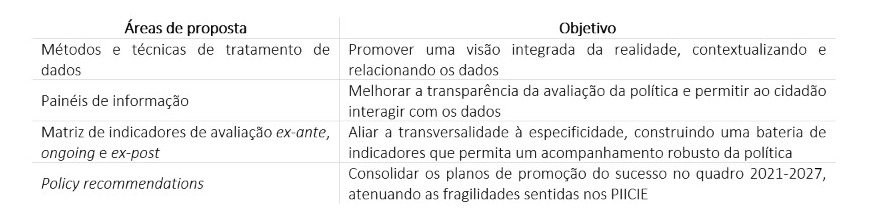
\includegraphics{C:/Users/julio/Documents/bookPoat/imagensRelatorio/f2017e0e-c5d0-4088-b8a1-78d738a5e183.jpg}

\begin{figure}
\centering
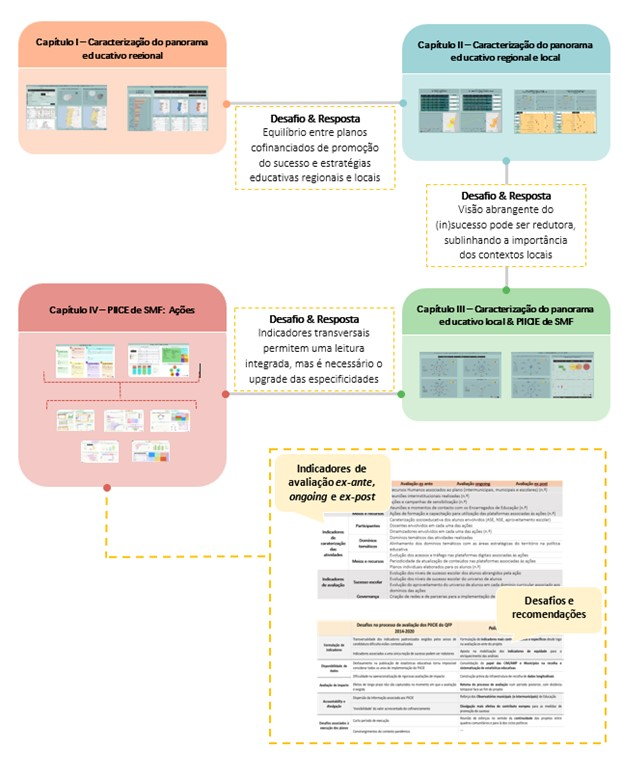
\includegraphics{C:/Users/julio/Documents/bookPoat/imagensRelatorio/Imagem1.jpg}
\caption{FIGURA 1: Diálogo proposto entre Painéis de Informação, Indicadores de Avaliação e Recomendações na implementação de estratégias de monitorização do (in)sucesso escolar - FONTE: GETIN-UA}
\end{figure}

\hypertarget{metodologia}{%
\section{Metodologia}\label{metodologia}}

Este projeto adota, ainda assim, uma metodologia que parte de indicadores mais genéricos (associados aos indicadores de resultado e realização dos Programas Operacionais) e propõe indicadores específicos para as ações. Procura privilegiar-se a territorialização e contextualização dos indicadores, ainda que partindo daqueles mais padronizados. A informação será apresentada através de painéis que surgem como exemplificativos de uma estratégia de tratamento e apresentação de dados que permita situar o território (face a outras unidades territoriais) e caracterizá-lo, do ponto de vista da implementação deste projeto específico (o PIICIE). \textbf{Idealmente, a construção dos \emph{dashboards} seria feita por meio da interoperabilidade de sistemas, assumindo que a informação a preencher pelas escolas (quer para a tutela, quer para a autoridade de gestão dos fundos comunitários) pode ser mobilizada, ao invés de multiplicada.}

\hypertarget{construuxe7uxe3o-dos-dashboards}{%
\subsection{\texorpdfstring{Construção dos \emph{dashboards}}{Construção dos dashboards}}\label{construuxe7uxe3o-dos-dashboards}}

Para Wickhan e Grolemund (2019, p.~473), \emph{dashboards} são uma maneira favorável de comunicar grandes quantidades de informação visualmente e rapidamente. Gartner (2020, p.~1) destaca que os dashboards agregam indicadores de desempenho (KPIs), tornando possível serem utilizados rapidamente por todos os utilizadores antes de uma eventual exploração adicional através de ferramentas de análise. Os \emph{dashboards} apresentam a informação combinando texto e opções gráficas num painel. Na maiorias das vezes, são as opções gráficas que acabam por se destacar, pois, comunicam a informação de forma mais inteligível.

Na etapa de tratamento e análise de dados, que precede a construção dos \emph{dashboards}, utilizou-se o \emph{software} estatístico R. Este \emph{software} é uma linguagem e ambiente para computação estatística e representação visual da informação tratada, permitindo aplicar uma ampla variedade de métodos (e.g.~modelação linear e não linear, testes estatísticos clássicos, análise de séries temporais, classificação, agrupamento). Para a construção dos dashboards utilizou-se a ferramenta \emph{Microsoft Power BI}. Segundo a informação disponível no sítio da \emph{Microsoft}, o \emph{Power BI} é uma coleção de serviços de \emph{software}, aplicações e conectores que funcionam em conjunto para transformar as origens de dados não relacionadas em informações coerentes, visualmente envolventes e interativas. O \emph{Power BI} permite ligar-se facilmente às origens de dados, visualizar e descobrir o que é importante, bem como partilhar os seus conteúdos com qualquer pessoa.

\begin{figure}
\centering
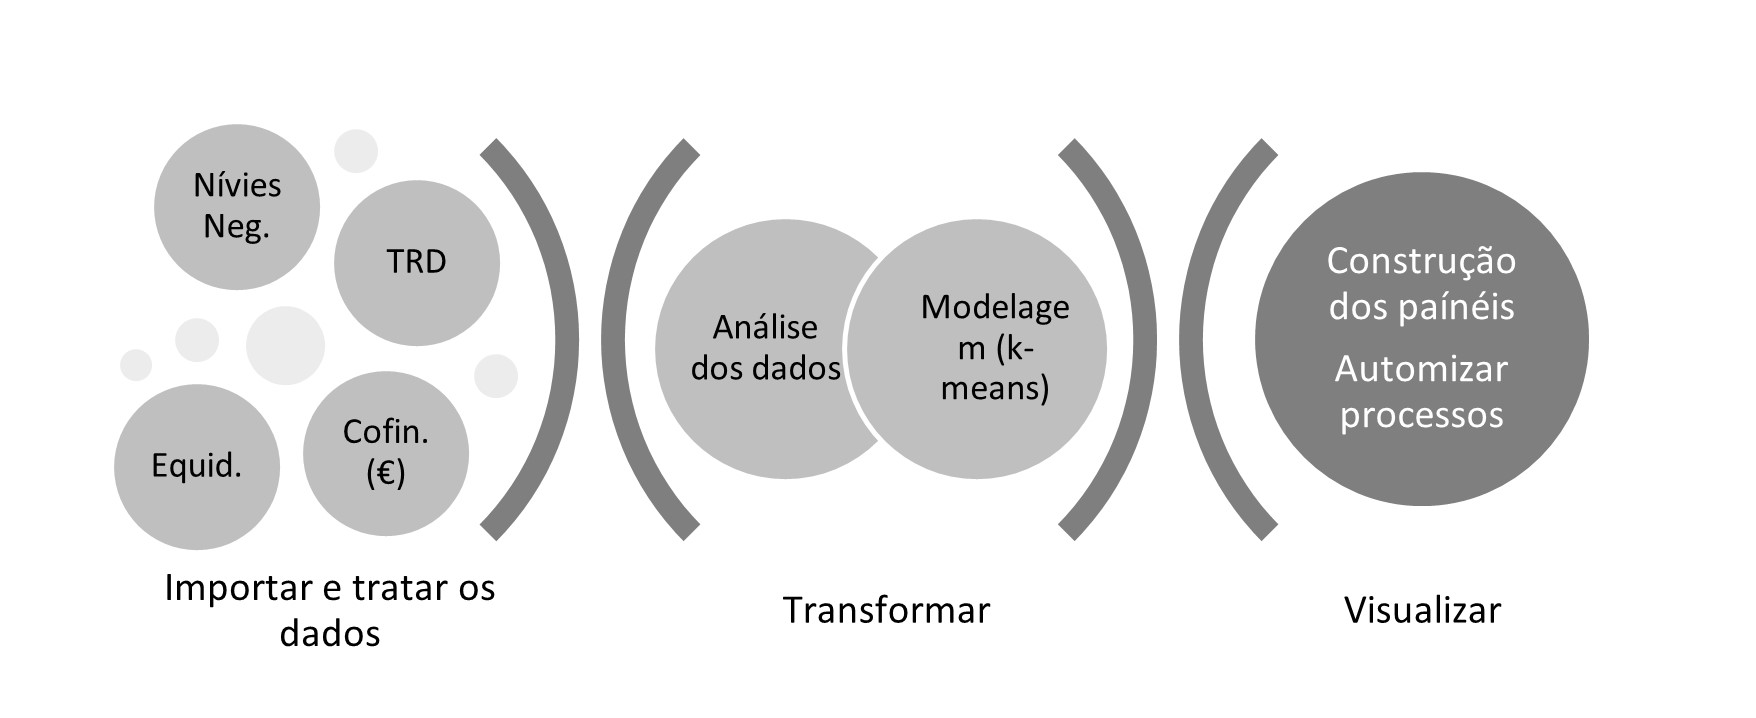
\includegraphics{C:/Users/julio/Documents/bookPoat/imagensRelatorio/Imagem2.jpg}
\caption{FIGURA 2: O ciclo da Ciência dos Dados - FONTE: Wickhan e Grolemund (2019)}
\end{figure}

A figura anterior apresenta as etapas dos processos de recolha, tratamento e análise de dados nacionais sobre o (in)sucesso escolar, numa perspetiva de utilização das ferramentas computacionais de maneira intercooperativa e multiplataforma. Grande parte dos dados disponibilizados para a análise estavam distribuídos em diversas plataformas eletrónicas, diferentes suportes de armazenamento de dados e estruturas de dados também elas distintas (fazer referência às mais importantes). Este formato não se mostrou ser o ideal para os objetivos do projeto, colocando desafios em diferentes etapas da sua concretização. Foi necessário um esforço adicional no tratamento de dados, de modo a transformá-los numa estrutura triangular, tanto para a construção de \emph{dashboards}, quanto para a modelação matemática proposta.

\hypertarget{diagnuxf3stico-do-insucesso-escolar}{%
\subsection{Diagnóstico do (in)sucesso escolar}\label{diagnuxf3stico-do-insucesso-escolar}}

\textbf{Tendências e padrões no sucesso}

O diagnóstico de tendências e padrões ao nível do sucesso escolar foi desenvolvido tendo como objetivo último caracterizar o território de estudo -- o município de Santa Maria da Feira (SMF). As análises produzidas nos diferentes capítulos dos dashboards refletem-se nos painéis de informação elaborados (2 painéis por capítulo). A caracterização do panorama educativo parte assim de uma visão geral do território nacional, para as regiões de referência de SMF, a Região Norte (NUTSII) e a Área Metropolitana do Porto (NUTS III), afunilando no contexto específico do município.

\textbf{1. Capítulo I - Caracterização do panorama educativo nacional}

O capítulo I desenvolve-se em torno do mapeamento do indicador de cofinanciamento (1º painel) e de uma análise de similaridades, que combina indicadores gerais de resultado com outros indicadores de caracterização socioeducativa relevantes na definição de clusters territoriais (2º painel).
O indicador de cofinanciamento foi incorporado no modelo seguindo critérios de distribuição dos recursos em M/€ correspondentes às operações PIICIE aprovadas, intermunicipais e municipais. Neste exercício foram considerados os valores alocados diretamente aos municípios, juntamente com o resultado do rácio dos recursos intermunicipais (NUTSIII). A incorporação no modelo segue a proporcionalidade de alunos em cada nível de ensino.\\
Já a análise de similaridades, ou de agrupamento, permitiu formar clusters territoriais, que decorrem do reconhecimento de semelhanças entre municípios de Portugal Continental, recorrendo até 4 indicadores de 2017/18 a 2019/20: i) total de alunos, ii) média das taxas de retenção e desistência (TRD), iii) equidade e iv) rácio entre cofinanciamento de operações PIICIE e total de alunos do ensino básico, ensino secundário em cursos científico-humanísticos (CCH) e em cursos profissionais (Prof.). Duas análises de similaridade foram realizadas, com representações gráficas que permitem confrontar as diferenças ao nível da formação dos clusters: a similaridade 1, que considera o total de alunos (eixo dos YY), a TRD (eixo dos XX) e a equidade (tamanho da bola); e a similaridade 2, que inclui os indicadores de cofinanciamento (eixo dos YY), da TRD (eixo dos XX) e da equidade (tamanho da bola).\\
A análise de similaridades pode ser entendida como um processo que permite descobrir relações existentes entre os exemplares de um conjunto de dados descritos por uma série de características (atributos descritivos). As análises realizadas pelos algoritmos que implementam estratégias para agrupamento procuram por similaridades ou diferenças entre exemplares, qualificadas através de medidas de distância (quanto menor for a distância entre dois exemplares, maior será a similaridade). Assim, exemplares similares serão associados a um mesmo grupo e exemplares dissimilares a grupos diferentes. No final de um algoritmo de agrupamento, uma estrutura será formada de maneira a que a similaridade intragrupos tenha sido maximizada e a similaridade intergrupos minimizada. Este estudo utiliza o \emph{k-means}, que agrupa os dados em grupos de variância igual em relação aos pontos médios, chamados centróides (Silva, Peres e Boscarioli, 2021 \& Sampaio, 2018).

\textbf{2. Capítulo II - Caracterização do panorama educativo regional e local }

Ao nível do capítulo II, duas análises estiveram na base da elaboração dos painéis de informação partindo dos indicadores gerais de resultado indicados no aviso de candidatura do PIICIE: i) uma análise regional dos municípios da Área Metropolitana do Porto (AMP), ao nível das Taxas de Níveis Negativos (TNN) a pelo menos uma disciplina e das Taxas de Retenção e Desistência (TRD) (1º painel); e ii) uma análise à escala local dos 9 Agrupamentos de Escolas (AE) do município de SMF (2º painel).\\
Para esta análise, foram utilizadas bases de dados estatísticos de diferentes instituições oficiais, que cobrem períodos distintos e com diferentes níveis de desagregação. Os dados relativos aos alunos com níveis negativos apenas estavam disponíveis para os 17 municípios da AMP (NUTSIII), de 2014/2015 a 2019/2020, desagregados por escola e para o 2º e 3º CEB. Já a informação relativa aos alunos retidos e desistentes, abrangiam todos os municípios da Região Norte (NUTSII), num total de 86 municípios, de 2014/2015 a 2018/2019, desagregada também por escola para todos os níveis do Ensino Básico e Secundário. No 1º painel, optou-se por modelar os dados e apresentar os indicadores apenas para os territórios da AMP, permitindo a respetiva análise e espacialização à escala da NUTSIII e seus municípios, numa perspetiva comparada. A espacialização dos dois indicadores gerais de desempenho é condicional às respetivas unidades temporais. Além dos dados da AMP, no 2º painel, é possível a análise e espacialização das TNN e TRD por AE do município de estudo e suas escolas.

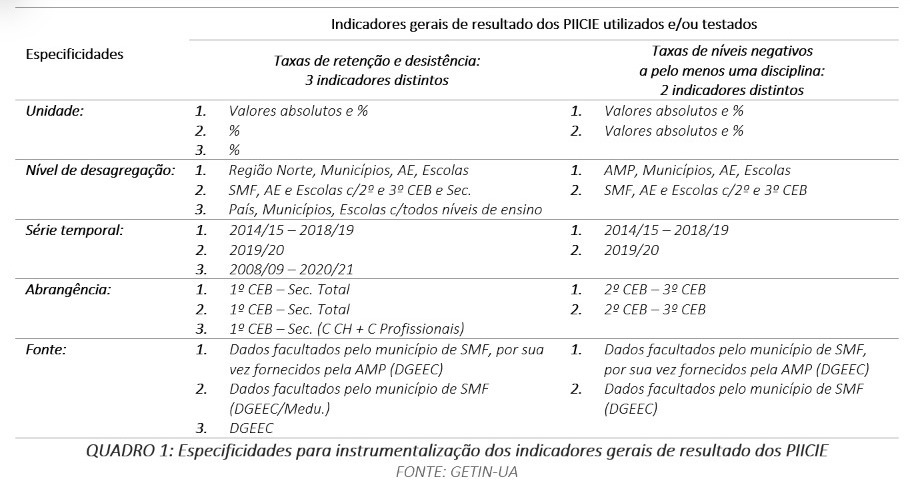
\includegraphics{C:/Users/julio/Documents/bookPoat/imagensRelatorio/quadro1.jpg}

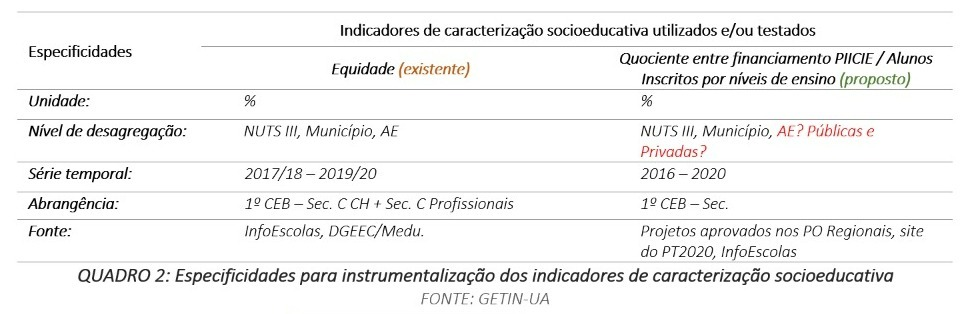
\includegraphics{C:/Users/julio/Documents/bookPoat/imagensRelatorio/quadro2.jpg}
HR -- 1) descrição sucinta dos princípios metodológicos da análise estatística inicial:\\
- Taxas de retenção e desistência
- Taxas de níveis negativos a pelo menos uma disciplina.

A análise concentrou-se, principalmente, em dois indicadores: Níveis Negativos (NN) e Retenção e Desistência (RD). Foram utilizadas bases do governo central de Portugal, disponíveis em diferentes sítios oficiais. As estatísticas disponíveis cobrem períodos distintos e possuem diferentes de níveis de desagregação. A análise dos Níveis Negativos considerou os 17 municípios da Área Metropolitana do Porto, entre 2014/2015 a 2019/2020, desagregados por escola e para o 2º e 3º anos do Ciclo Básico. Já a Retenção e Desistência, cobrem a região Norte (NUTS-III), o que corresponde a 86 municípios, entre 2014/2015 a 2018/2019 e possuem desagregação dos dados para todos os anos escolares do Ciclo Básico e Secundário. Os indicadores foram analisados separadamente e, quando necessária a análise conjunta, seja para efeito de comparação ou modelagem, estes ficaram restritos às unidades espaço-temporais comuns que contemplavam os dois indicadores. Além dos dados da AMP, foram analisados os dados de Níveis Negativos e Retenção e Desistência do município de Santa Maria da Feira.

HR -- 2) descrição sucinta dos princípios metodológicos da análise de similaridades:
- Clusters fase 1: alunos c/Níveis Negativos, Retidos, Inscritos e c/ASE
- Cluster fase 2: combinação de TRD (País?) + financiamentos + equidade

\textbf{Análise de agrupamentos (clusterização)}

Análise de agrupamento pode ser entendida como um processo que permite descobrir relações existentes entre os exemplares de um conjunto de dados descritos por uma série de características (atributos descritivos). Em geral, as análises realizadas pelos algoritmos que implementam estratégias para agrupamento buscam por similaridades ou diferenças entre exemplares, qualificadas por meio de medidas de distância (quanto menor for a distância entre dois exemplares, maior será a similaridade), tal que exemplares similares sejam associados a um mesmo grupo, e exemplares dissimilares, a grupos diferentes. Ao final da execução de um algoritmo de agrupamento, uma estrutura de grupo é formada de maneira que a similaridade intragrupos tenham sido maximizadas, e a similaridade intergrupos tenha sido maximizada. Este estudo utiliza o \emph{k-means}, que agrupa os dados em grupos de variância igual com relação aos pontos médios, chamados centroides. (Silva, Peres e Boscarioli, 2021 \& Sampaio, 2018). A formação dos \emph{clusters} obedeceu a menor estrutura de dados comuns às variáveis consideradas na busca por similaridades.

Em uma etapa posterior, foram consolidados dados de todo o país da população estudantil, taxa de retenção e desistência e equidade, com o objetivo de identificar padrões entre as diversas regiões do país, ao considerar essas três variáveis. Estes dados estão desagregados por nível de ensino, ciclo de estudos, ano de escolaridade, NUTS II, NUTS III de 2013 e município.

\textbf{Fatores de influência do sucesso}

A análise de autocorrelação espacial foi aplicada aos municípios da Região Norte -- NUTS II de referência do município de estudo -- e contribuiu para a identificação de possíveis fatores de influência do sucesso escolar nesses territórios. De forma sucinta, a análise desenvolvida consiste em perceber a influência de municípios vizinhos no comportamento de uma determinada variável dependente num município específico e apurar quais os fatores que melhor permitem explicar o comportamento dessa variável -- neste caso, foram analisadas as taxas de retenção e desistência. Através da linguagem de programação Python, foi possível realizar vários testes e modelar a dependência espacial das taxas de retenção e desistência por via de uma análise de regressão espacial.\\
A opção de analisar as taxas de retenção e desistência enquanto indicador geral de resultado dos PIICIE, na catação de possíveis fatores de sucesso, decorreu do facto da informação estar disponível para todos os municípios da Região Norte, enquanto para as taxas de níveis negativos a pelo menos uma disciplina só foi possível aceder a dados para os municípios da AMP com igual desagregação. A análise reporta a 2018/19, tendo sido realizada para o ensino básico (1º, 2º e 3º CEB) e secundário das escolas públicas agrupadas.\footnote{Para consulta da respetiva fonte, ver Quadro 1.} Em municípios com mais de um agrupamento de escolas (AE), os dados foram agregados.\\
Na base da seleção das variáveis independentes, assumiu-se como critério chave a sua relevância para a leitura espacial, demográfica, socioeconómica e socioeducativa dos territórios a analisar, com desagregação até ao município. No total, foram consideradas 16 variáveis explicativas\footnote{A informação utilizada tem origem em bases de dados abertas do PORDATA (variáveis recolhidas -- densidade populacional, nº de estabelecimentos de ensino ativos em cada nível, população que completou o ensino secundário e o ensino superior, poder de compra per capita) e Infoescolas (variáveis recolhidas -- equidade e percentagem de alunos com ASE que concluíram os níveis de ensino básico e secundário nos anos previstos).
  Para maior detalhe sobre os indicadores de equidade e alunos com ASE, ver o Quadro 2.}:

\begin{itemize}
\tightlist
\item
  densidade populacional referente ao ano de 2021 (valores previstos) - 1 variável;
\item
  percentagem de estabelecimentos de ensino ativos em cada nível (excluindo o ensino pré-escolar) face ao total no ano de 2019/20 -- 4 variáveis;
\item
  percentagem de indivíduos que completou o ensino secundário e o ensino superior face ao total de residentes em 2011 -- 2 variáveis;
\item
  poder de compra per capita registado em 2019 -- 1 variável;
\item
  indicador de equidade referente aos níveis de ensino básico e secundário (média entre o científico-humanísticos e profissional) -- 4 variáveis;
\item
  percentagem de alunos com ASE que concluíram os níveis de ensino básico e secundário (média entre o científico-humanísticos e profissional) nos anos previstos - 4 variáveis
\end{itemize}

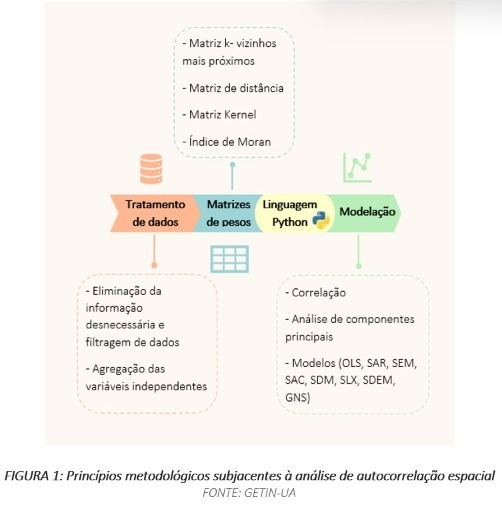
\includegraphics{C:/Users/julio/Documents/bookPoat/imagensRelatorio/figura1.jpg}\\
Na Figura 1 esquematiza as três principais etapas da análise de autocorrelação espacial desenvolvida\footnote{Para maior detalhe, consultar o ponto 2.3.}:
\textbf{1.} a 1ª fase centrou-se no tratamento de dados e teve como objetivo recolher a informação essencial para a análise -- as variáveis dependentes e independentes;\\
\textbf{2.} na 2ª fase o propósito passou por encontrar a melhor matriz de pesos através do cálculo do índice de Moran. A abordagem utilizada para a representação das interações espaciais incluiu o teste de três tipos de matrizes de pesos espaciais -- matriz de distância de 100 km, matriz k-vizinhos mais próximos e matriz de Kernel -- sendo estas matrizes de pesos baseadas em distâncias. As matrizes representam as interações espaciais entre diferentes objetos, neste caso entre os diversos municípios. Em particular, as matrizes de distância permitem definir as relações de vizinhança em função da distância entre os municípios. A matriz de distância de 100 km é um tipo de matriz de distância mais simples, tendo sido pré-estabelecido uma distância que irá funcionar como uma ordem de nível para a definição dos vizinhos. Na matriz k-vizinhos define-se exatamente o número de vizinhos mais próximos de cada município, ou seja, todos os municípios têm o mesmo número de vizinhos. A matriz Kernel é modulada por uma função de Kernel com determinadas propriedades, sendo que os pesos entre os municípios são baseados na sua distância. Em cada matriz foi calculado o índice de Moran geral e local para escolher a aquela que melhor traduzisse as interações espaciais entre os municípios da Região Norte. Com base no índice de Moran local, construiu-se também o diagrama de dispersão;\\
\textbf{3.} por fim, a 3ª fase consistiu em analisar a correlação entre as diferentes variáveis, dependentes (4 variáveis) e independentes/explicativas (16 variáveis), e chegar ao modelo que melhor permitisse inferir sobre as relações de influência e causalidade. Esta etapa compreendeu a elaboração de uma autocorrelação (anterior à análise de componentes principais) e a modelação das variáveis através de uma análise de componentes principais.\\
Para além da análise da correlação entre as variáveis, a análise de componentes principais permitiu a obtenção de um pequeno número de combinações lineares das 18 variáveis utilizadas que representem a maior parte da variabilidade dos dados. Este tipo de análise tornou-se útil para modelar a dependência espacial.\\
Foi possível aferir que quatro fatores seria o nº mais adequado para realizar a análise de componentes principais. Desta forma, analisando os resultados obtidos dos loadings, verifica-se que o fator 1 tem mais influência na variável relativa ao poder de compra, dado que o valor se encontra próximo de 1 ou de -1 (0,88). Algo semelhante ocorre com os restantes fatores, sendo que exercem mais influência nas variáveis relativas à percentagem de estabelecimentos do 2ºCEB ativos (0,60), equidade referente ao secundário (0,49) e percentagem de alunos com ASE que concluíram o 2ºCEB nos 3 anos (0,77), respetivamente. Estas quatro variáveis foram utilizadas na construção dos modelos testados.\\
É possível avaliar a presença de dependência espacial através de um vasto conjunto de modelos, sendo que se verificou qual seria o melhor modelo para cada um dos níveis de ensino. Assim, assume-se que o melhor modelo para todos os níveis de ensino é o modelo OLS, dado que ao realizar este modelo nenhum multiplicador de Lagrange (LM-Error e LM-Lag) têm significância devia às fracas autocorrelações observadas entre as variáveis desfasadas e o desvio padrão de cada nível de ensino.

\hypertarget{desconstruuxe7uxe3o-do-piicie-de-smf}{%
\subsection{Desconstrução do PIICIE de SMF}\label{desconstruuxe7uxe3o-do-piicie-de-smf}}

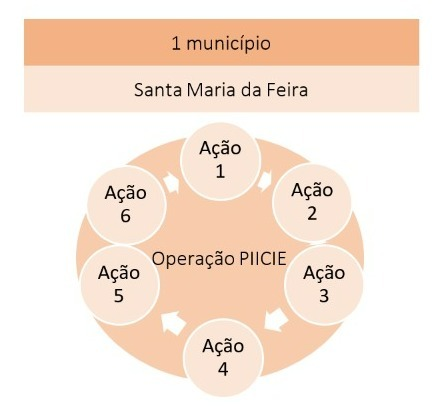
\includegraphics{C:/Users/julio/Documents/bookPoat/imagensRelatorio/figura2.jpg}\\
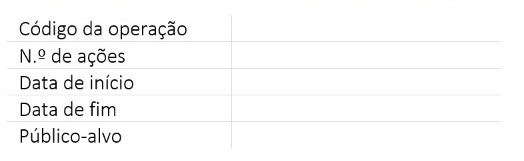
\includegraphics{C:/Users/julio/Documents/bookPoat/imagensRelatorio/figura3.jpg}

O PIICIE de Santa Maria da Feira surge em resposta ao aviso de candidatura XXXXX. Recorrendo ao jargão europeu, na sequência desta candidatura foi financiada uma única operação que, por sua vez, se desdobra em várias ações. Por oposição, há outras entidades beneficiárias que gerem um PIICIE cujas ações correspondem a diferentes operações cofinanciadas.

Em Santa Maria da Feira, cada uma das 6 ações compreendidas na operação cumpre um propósito distinto e enquadra-se em diferentes domínios temáticos. Esta diversidade deve ser tida em conta aquando da formulação de indicadores que devem combinar a transversalidade com a especificidade.

Em jeito introdutório, cada uma das ações do PIICIE de Santa Maria da Feira pode ser resumida através de uma palavra ou expressão, algumas remetendo para os princípios subjacentes, outras para os domínios temáticos:

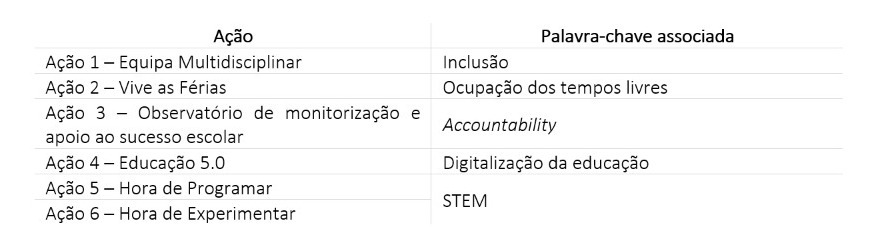
\includegraphics{C:/Users/julio/Documents/bookPoat/imagensRelatorio/figura4.jpg}

Por outro lado, há ações que têm uma abrangência de público declaradamente alargada, como a Ação 2 -- Vive as Férias ou, no limite, a Ação 3 -- Observatório, cuja plataforma de consulta pública deveria ser visitada por todos os munícipes que assim desejassem. Por outro lado, a Ação 1 -- Equipa Multidisciplinar compreende um rigoroso processo de seleção dos alunos a incluir nas atividades; a Ação 6 -- Hora de Experimentar destina-se a alunos de apenas 4 dos 9 Agrupamentos de Escolas\footnote{Sublinhe-se, desde já, que a Hora de Experimentar foi alargada aos restantes Agrupamentos de Escolas, ainda que sem cofinanciamento europeu, sendo as despesas assumidas pela autarquia.}.

\hypertarget{acessos-consulta-e-divulgauxe7uxe3o}{%
\subsection{Acessos, consulta e divulgação}\label{acessos-consulta-e-divulgauxe7uxe3o}}

HR -- 1) descrição sucinta dos passos instrumentais para o acesso, consulta e divulgação dos trabalhos:
Apresentação dos diretórios/instruções para consulta e divulgação dos dashboards
Descrição dos passos para criação e disponibilização do relatório online.

{[}Disponibilização de arquivos compactado com o projeto completo, contendo: Dados originais, base de dados tratados, códigos em R utilizados no processo de ETL, do inglês Extract, Transform, Load (Extrair Transformar Carregar) e do modelo não supervisionado de Machine Learning (K-Means) para a formação de clusters, além de um arquivo desenvolvido em Power BI, este último, a conter, efetivamente, o dashboard. {]}\\
As evidências reunidas, dada a informação desagregada à qual foi possível aceder, centram-se nos municípios da Região Norte e, em particular, da Área Metropolitana do Porto (AMP) -- NUTS II e NUTS III de referência da unidade territorial de estudo, o município de Santa Maria da Feira. Encontram-se estruturadas em dois pontos: 1) análise estatística inicial dos indicadores gerais de resultado indicados no aviso de candidatura dos PIICIE e 2) análise de similaridades entre municípios (clusters territoriais) cruzando os indicadores gerais de desempenho e indicadores de caracterização socioeducativa.

HR -- 1) descrição sucinta dos resultados com base na análise estatística inicial:\\
Taxas de retenção e desistência
Taxas de níveis negativos a pelo menos uma disciplina

{[}por fazer{]}

HR -- 2) descrição sucinta dos resultados com base na análise de similaridades:
Clusters fase 1: alunos c/Níveis Negativos, Retidos, Inscritos e c/ASE
Cluster fase 2: combinação de TRD + financiamentos + equidade

{[}por fazer{]}

\hypertarget{possuxedveis-fatores-de-influuxeancia}{%
\section{Possíveis fatores de influência}\label{possuxedveis-fatores-de-influuxeancia}}

A análise aqui desenvolvida abrange os municípios da Região Norte e permite tecer algumas conclusões acerca da influência destas unidades espaciais no comportamento das taxas de retenção e desistência das unidades vizinhas. A identificação de associações espaciais entre os municípios decorreu da análise i) de matrizes de pesos (k-vizinhos mais próximos, de distância a 100km e de Kernel), ii) do cálculo do Índice de Moran para cada matriz (para avaliar a existência de autocorrelação espacial) e iii) da representação dos diagramas de dispersão de Moran e dos mapas LISA:

\begin{itemize}
\tightlist
\item
  O Índice de Moran é um indicador que permite aferir a semelhança geral entre regiões (neste caso, são considerados municípios). Quanto mais próximo de 1 for este índice, mais adequada será a utilização da matriz, devendo o seu nível de significância (p-sim) ser \textless{} 5\%;
\item
  Os diagramas de dispersão de Moran partem do cálculo do índice de Moran e, num referencial de 4 quadrantes, permitem visualizar a desfasagem espacial da variável das taxas de retenção e desistência (eixo dos y) e o desvio padrão desse mesma variável (eixo dos x). As autocorrelações (associações espaciais) positivas-fortes implicam semelhanças entre municípios vizinhos, as negativas-fortes traduzem dissemelhanças e as autocorrelações fracas refletem ausência de associação espacial:
\end{itemize}

\textbf{Quadrante Alto-Alto (Q1)}: municípios e vizinhos com valores elevados da taxa de retenção e desistência;
\textbf{Quadrante Baixo-Alto (Q2)}: municípios com valores baixos e vizinhos com valores elevados da taxa de retenção e desistência;
\textbf{Quadrante Baixo-Baixo (Q3)}: municípios e vizinhos com valores baixos da taxa de retenção e desistência;
\textbf{Quadrante Alto-Baixo (Q4)}: municípios com valores elevados e vizinhos com valores baixos da taxa de retenção e desistência;

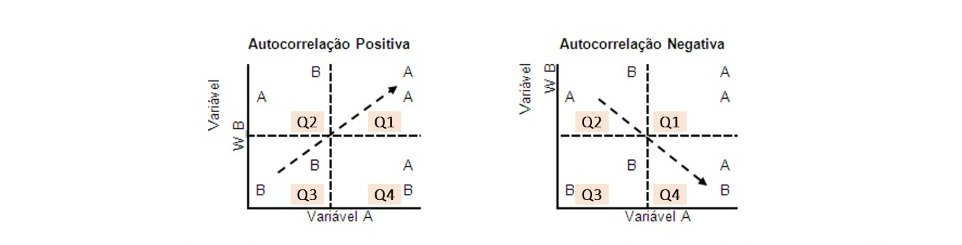
\includegraphics{C:/Users/julio/Documents/bookPoat/imagensRelatorio/figura9.jpg}

\begin{itemize}
\tightlist
\item
  Os mapas LISA traduzem espacialmente os resultados dos digramas de dispersão de Moran. As cores presentes, tanto no diagrama de dispersão de Moran como no mapa LISA, representam os quatro tipos de dependências relacionais entre vizinhos referidos anteriormente - vermelho: ``High-High'' (municípios e vizinhos com valores elevados da taxa de retenção e desistência); azul claro: ``Low-High'' (municípios com valores baixos e vizinhos com valores elevados da taxa de retenção e desistência); azul escuro: ``Low-Low'' (municípios e vizinhos com valores baixos da taxa de retenção e desistência); laranja: High-Low (municípios com valores elevados e vizinhos com valores baixos da taxa de retenção e desistência); cinza: municípios que não são significantes para a análise.
\end{itemize}

Na \textbf{FIGURA 5} estão representados os diagramas de dispersão de Moran e os mapas LISA obtidos com a matriz de Kernel para o 1ºCEB e com a matriz k-vizinhos mais próximos para os restantes níveis de ensino, sendo que estas foram aquelas que se destacaram entre as matrizes de pesos calculadas, dado o Índice de Moran ter sido mais expressivo. As autocorrelações positivas e negativas podem ser fracas ou fortes. Neste sentido, é importante analisar o índice de Moran das matrizes selecionadas, de modo a perceber se este se encontra próximo de 1 (autocorrelações positivas e negativas fortes). Assim, as autocorrelações correspondentes 2ºCEB, 3ºCEB e Secundário são positivas fracas e no 1ºCEB a autocorrelação é negativa fraca, apresentando valores do Índice de Moran afastados de 1. Ainda na \textbf{FIGURA 5} , encontra-se os mapas LISA e o mapeamento da variável dependente, a taxa de retenção e desistência de cada nível de ensino.

Como é possível deduzir através do mapa LISA relativamente à Taxa de Retenção e Desistência do 1ºCEB, Tarouca é assinalada como um município que apresenta valores elevados desta variável, ao contrário dos municípios vizinhos que têm valores baixos. Neste caso, o município não aparenta ser influenciado pelos valores apresentados pelos vizinhos, uma vez que estes têm um comportamento oposto.

Os municípios da Maia, do Porto e de Gondomar apresentam valores elevados de taxas de retenção e desistência do 2ºCEB, verificando-se uma influência evidente entre estes e os municípios vizinhos que apresentam igualmente valores elevados. Ainda relativamente a esta variável, Valpaços não é afetado pelos valores obtidos pelos vizinhos, sendo que este município apresenta valores elevados e os seus vizinhos não.

No 3ºCEB, verifica-se influência entre os municípios de Vila do Conde, Matosinhos, Maia, Porto e Gondomar e os seus vizinhos, pois todos apresentam valores elevando da taxa de retenção e desistência. Já Bragança tem um comportamento contrário aos seus vizinhos, obtendo valores baixos, enquanto os seus vizinhos têm valores altos. Os municípios de Ponte da Barca e Vila Verde, assim como os seus vizinhos, têm valores baixos da taxa de retenção e desistência do 3ºCEB.

Na taxa de retenção e desistência do secundário, Matosinhos, Porto e Gondomar são municípios que têm valores elevados, tal como os municípios à sua volta, verificando-se uma clara influência. O município de Celorico de Basto apresenta valores elevados, contrariamente aos valores da taxa de retenção e desistência apresentados pelos vizinhos. Miranda do Douro posiciona-se numa situação oposta a Celorico de Basto, pois apresenta valores baixos da taxa de retenção e desistência do secundário, enquanto os seus vizinhos têm valores elevados desta variável. Nestes dois municípios, é fácil de deduzir que não existe influência entre estes e os seus vizinhos.

\begin{itemize}
\item
  Era interessante criar uma tabela para cada nível de ensino e listar os municípios por quadrante em função do tipo de autocorrelação. Para ser mais simples identificar.
\item
  O Município de SMF aparece sempre a cinza. Refletir a respeito.
\end{itemize}

JM: Apesar de se encontrar a cinza, isto é, não é significante para a análise, uma vez que, como está acima referido para a TRD do 2ºCEB, 3º CEB e Secundário, grande parte dos municípios da AMP estão a vermelho, isto é, são municípios que têm valores elevados e os seus vizinhos também. Desta forma, pode deduzir que pelo menos para estes níveis de ensino, SMF apresenta valores elevados.

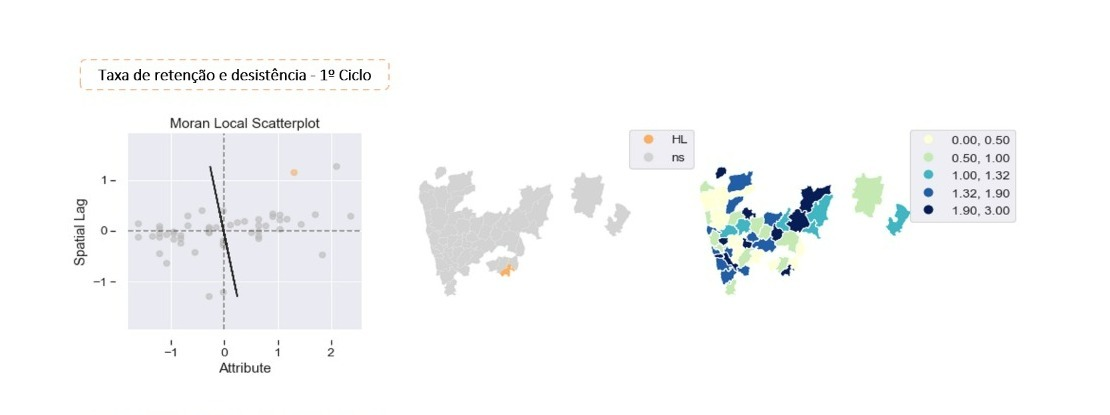
\includegraphics{C:/Users/julio/Documents/bookPoat/imagensRelatorio/figura10.jpg}\\
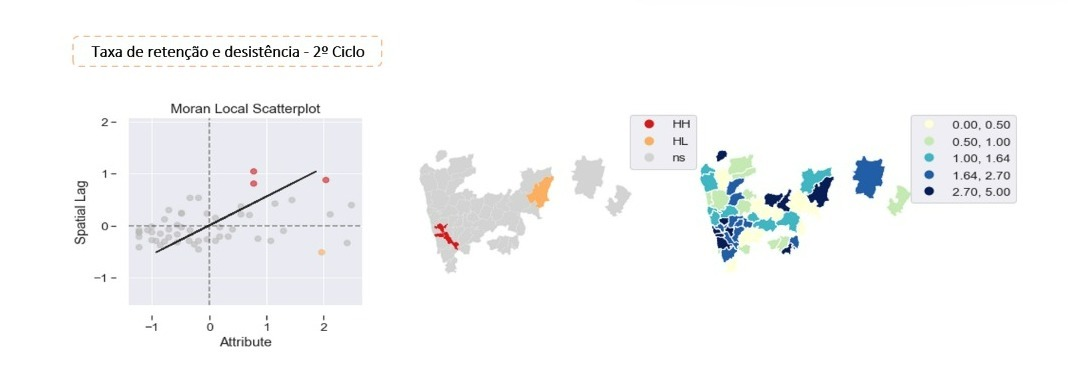
\includegraphics{C:/Users/julio/Documents/bookPoat/imagensRelatorio/figura11.jpg}\\
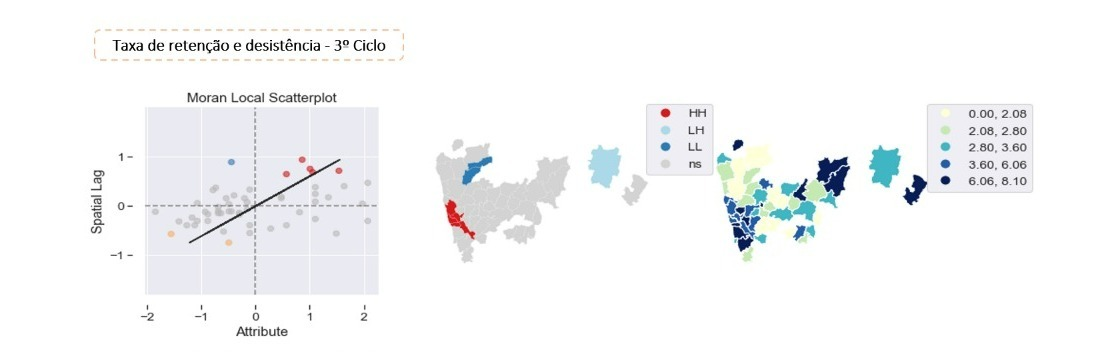
\includegraphics{C:/Users/julio/Documents/bookPoat/imagensRelatorio/figura12.jpg}\\
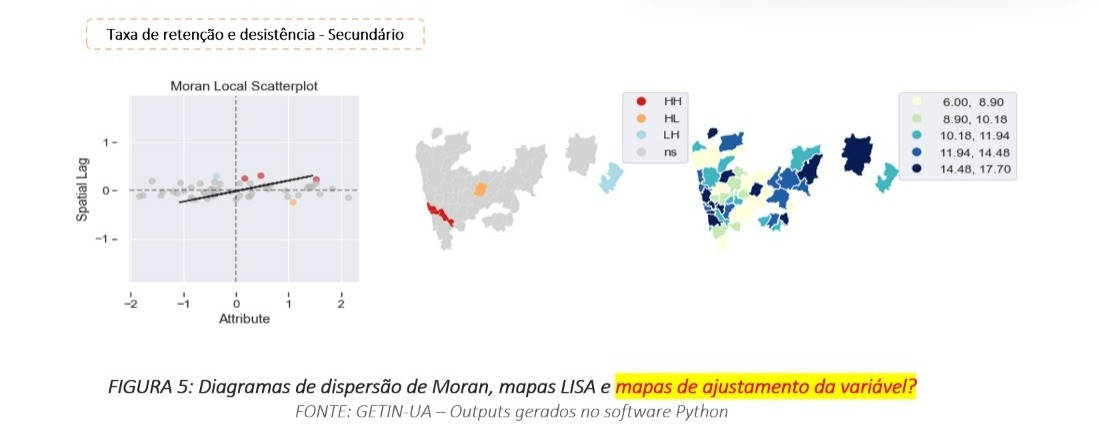
\includegraphics{C:/Users/julio/Documents/bookPoat/imagensRelatorio/figura13.jpg}

De forma a identificar possíveis fatores de influência relativamente à taxa de retenção e desistência de cada nível de ensino, adicionou-se à análise anteriormente mencionada um conjunto de variáveis. Assim, foi possível analisar a matriz de autocorrelação entre as taxas de retenção e desistência e as variáveis independentes/explicativas (FIGURA X).
JM: Escolher qual a matriz que irá ficar!

Inserir legenda\\
JM: talvez acrescentar uma legenda para identificar o significado das variáveis?

Facilmente, se retira algumas conclusões acerca de quais as variáveis que têm uma maior influência nas variáveis dependentes, as taxas de retenção e desistência. Todas as variáveis dependentes (TRD\_1CEB, TRD\_2CEB, TRD\_3CEB, TRD\_SEC) apresentam grande nível de correlação com a densidade e com o poder per capita. De salientar que também existe uma correlação evidente entre as taxas de retenção e desistência do 2ºCEB, 3ºCEB e secundário. Estas variáveis também apresentam maior correlação com percentagem de indivíduos que completou o ensino secundário e o ensino superior.\\
A variável da taxa de retenção do 1ºCEB, 2ºCEB e 3ºCEB têm uma correlação evidente com a percentagem de estabelecimentos de ensino ativos no 1ºCEB. Ainda é possível verificar que a taxa de retenção do 2ºCEB, 3ºCEB e secundário estabelecem uma correlação alta com a percentagem de alunos com ASE que concluíram o 2ºCEB nos 3 anos e com a equidade referente ao 2ºCEB.

\hypertarget{PIICIE}{%
\chapter{O PIICIE de Santa Maria da Feira}\label{PIICIE}}

\hypertarget{breve-caracterizauxe7uxe3o-territorial-e-educativa-do-municuxedpio}{%
\section{Breve caracterização territorial e educativa do município}\label{breve-caracterizauxe7uxe3o-territorial-e-educativa-do-municuxedpio}}

Ainda que Santa Maria da Feira tenha emergido como a unidade territorial em análise, o trabalho desenvolvido não se esgota na sua realidade, que deve ser entendida apenas como o ponto de partida. Não obstante, importa encetar uma breve caracterização, que permita conhecer o território em que se desenvolve o PIICIE em estudo.

O Município de Santa Maria da Feira é um território dinâmico e palco de diversidades que se traduzem na natureza plural dos seus territórios educativos. À semelhança de outros concelhos do país e das regiões onde se insere (AMP e Região Norte), enfrenta desafios i) que emergem de singularidades e assimetrias internas, i) que decorrem do panorama de evolução que se perspetiva para o médio e longo prazo e iii) que se enquadram em reptos mais abrangentes ligados a orientações nacionais e transnacionais. Assim, a compreensão das opções estratégicas na promoção do sucesso escolar em Santa Maria da Feira não poderá ser dissociada das características socioeducativas e dos referenciais de partida recentes na quantificação e interpretação dos níveis de desempenho que apresenta.

Com uma elevada dinâmica empresarial, associativa e cultural, bem como um forte histórico industrial, mais presente em algumas freguesias, o concelho de Santa Maria da Feira assinalou na última década uma evolução considerável dos níveis de qualificação da sua população residente (INE, 2021). As taxas de retenção, um dos principais indicadores abordados no estudo, pelo contrário, mostram uma diminuição e valores de referência abaixo dos da região e do país (confirmar) (DGEEC, 2022b). Ainda que estas sejam tendências transversais a vários territórios do país, importa sublinhar que a Educação tem sido assumida como área prioritária de intervenção no município de estudo, à qual tem sido dada crescente visibilidade. A candidatura realizada para elaboração do PIICIE municipal é disso exemplo, assim como o Projeto Educativo Municipal 2014'20 e mais recentemente o Plano Estratégico Educativo Municipal 2022-30, instrumentos que têm contribuído para a definição e afirmação das políticas educativas locais em articulação com outras áreas como a cultura, o desporto ou a economia.

A necessidade de acompanhar as respetivas dinâmicas e políticas educativas municipais tem conduzido, igualmente, a um investimento em medidas de monitorização, visando um olhar integrado sobre a implementação, o acompanhamento e a avaliação de projetos e iniciativas em matéria de educação, promovidas pelo município, mas também por outros agentes territoriais. Muitas destas iniciativas terão como objetivo específico promover o sucesso escolar, enquanto noutras o propósito será mais alargado e direcionado a outros domínios da área educativa, mas nem por isso menos relevantes na elevação e consolidação dos padrões de qualidade do sistema de ensino à escala local.

A riqueza e multiplicidades que povoam o concelho justificam a diversidade encontrada ao nível da rede educativa, da qual fazem parte, atualmente, 124 instituições desde a educação pré-escolar ao ensino superior (Marques et al., n.d.). A oferta pública conta com 85 estabelecimentos escolares distribuídos por 9 Agrupamentos de Escolas (AE). A escola de proximidade, isto é, aquela que corresponde aos primeiros níveis de educação e ensino (educação pré-escolar e 1º ciclo do ensino básico), é garantida nas 21 freguesias. E, naturalmente, que territórios centrais do concelho que têm registado, inclusive, um crescimento populacional coincidem com as áreas de influência dos agrupamentos de escolas com mais alunos inscritos, AE de Santa Maria da Feira e AE de Fernando Pessoa. Simultaneamente, várias instituições integram e contribuem para a qualificação da rede de ofertas educativas e formativas do concelho, como as instituições da rede solidária com educação pré-escolar, os centros de formação profissional públicos, as instituições privadas independentes do estado, as instituições de ensino artístico especializado, as instituições que salvaguardam a valência de creche e a instituição com oferta de ensino superior.

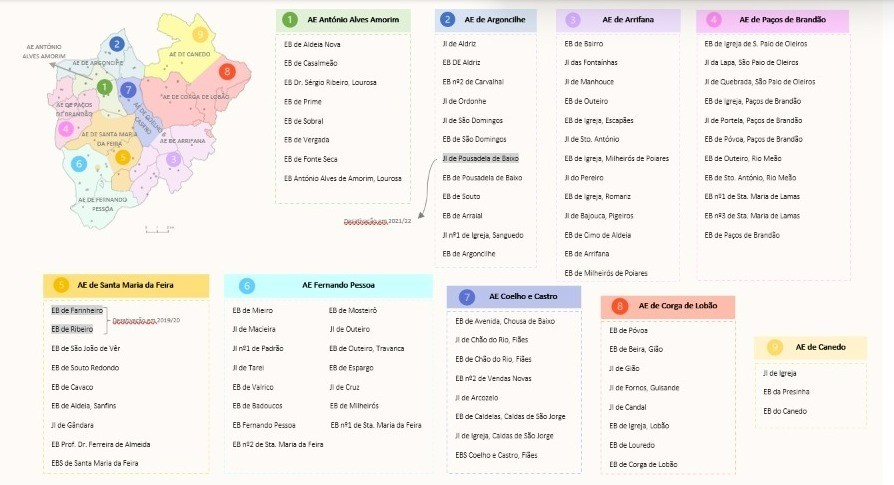
\includegraphics{C:/Users/julio/Documents/bookPoat/imagensRelatorio/figura14.jpg}

\hypertarget{apresentauxe7uxe3o-e-descriuxe7uxe3o-do-piicie}{%
\section{Apresentação e descrição do PIICIE}\label{apresentauxe7uxe3o-e-descriuxe7uxe3o-do-piicie}}

O PIICIE de Santa Maria da Feira denomina-se `EDUFEIR@ - Inovamos para o Sucesso' e integra seis ações que iniciaram a 12 de outubro de 2018 e terminaram a 31 de dezembro 2021. Como a Tabela X ilustra, as diferentes ações responderam a distintos desafios, decorrendo em períodos nem sempre coincidentes.

A \textbf{Ação 1 - Equipa Multidisciplinar} centra-se, essencialmente, na prevenção e na intervenção em casos de alunos que demonstram dificuldades em aprender e com risco de abandono escolar. \textbf{A Ação 2 - Vive as Férias} promove a aquisição de diversas competências ao nível individual e social, através de atividades lúdicas e criativas. A \textbf{Ação 3 - Observatório de Monitorização e Apoio ao Sucesso Escolar} foi criada com o objetivo de todos os munícipes conseguirem acompanhar de forma fácil e rigorosa as políticas educativas implementadas em Santa Maria da Feira. Já a \textbf{Ação 4 - Educação 5.0} foca-se no desenvolvimento de valores importantes para que as crianças, professores e pais tenham capacidades de exercerem um papel ativo na comunidade. Para além disso, esta ação pressupõe a criação de um ambiente tecnológico de modo a favorecer a partilha de informação e o trabalho colaborativo. A \textbf{Ação 5 - Hora de Programar} tem como princípios a inovação e a criatividade e é através destes princípios que pretende consolidar aprendizagens na área das ciências, matemática e leitura. Na \textbf{Ação 6 - Hora de Experimentar} são abordados fenómenos da natureza com o auxílio da ciência. Assim, os alunos têm oportunidade fazer experiências e, simultaneamente, aprender sobre ações do quotidiano.

Analisando a natureza e o espírito das ações de uma perspetiva global, destacam-se princípios como a cooperação e a colaboração, remetendo para o principal objetivo da criação do PIICIE, isto é, o foco no trabalho em rede para o desenvolvimento do município e para a capacitação da comunidade.

No total, participaram cerca de 18657 alunos nas ações do PIICIE (Figura 6).\footnote{Excetuam-se os participantes que poderiam estar associados à Ação 3, cuja contabilização não foi reunida.} A ação Educação 5.0 destaca-se com o maior número de participantes pelo facto de integrar tanto os participantes das Olimpíadas da Cidadania e do Património, nos anos de 2019/20 e 2020/21, como também todos os alunos envolvidos na atribuição de tablets às escolas no início de 2018. N.º total de alunos não coincide com dados relatório Cláudia. Verificar.
Três das principais mais-valias do PIICIE de Santa Maria da Feira passam pela diversidade temática dos domínios das ações, pela promoção da articulação interinstitucional e pela iniciativa municipal em dar continuidade temporal e estender o PIICIE a outros públicos para lá do cofinanciamento, assumindo a despesa. Aparenta, ainda, haver uma razoável visibilidade deste plano e entendimento em torno do seu valor.

\hypertarget{diversidade-temuxe1tica}{%
\subsection{\texorpdfstring{\textbf{Diversidade temática}}{Diversidade temática}}\label{diversidade-temuxe1tica}}

O desenho e implementação deste PIICIE assente em várias áreas temáticas traduz diferentes mensagens relevantes e que podem inspirar outros programas:
- 1) Entende-se que o combate ao insucesso escolar se faz por meio de diferentes tipologias de ação e que apenas uma abordagem simultaneamente multifacetada e integrada poderá ser bem-sucedida;
- 2) Ainda que alinhada com o discurso educativo da UE voltado para a sociedade baseada no conhecimento e para a competitividade (Nóvoa, 2013), a estratégia feirense aparenta ultrapassar esta visão estritamente económica e limitada da Educação. Confere, assim, atenção a matérias de inclusão, coesão e de trabalho junto da e para a comunidade.
- 3) A aposta estratégica em áreas STEM como centrais no sucesso escolar e pessoal dos indivíduos (ilustrada através das ações Hora de Experimentar e Hora de Programar).\\
Ainda que haja uma ligação entre o PIICIE e a estratégia local para a Educação, ficam de fora da espinha dorsal do projeto algumas áreas estratégicas de Santa Maria da Feira, como as Artes ou o Desporto, ainda que se entenda que estas são centrais para o sucesso escolar (REF PEEM). No entanto, esta opção limita as redundâncias e permite à política cofinanciada cumprir o seu valor acrescentado (Mairate, 2007).

\hypertarget{articulauxe7uxe3o-interinstitucional}{%
\subsection{\texorpdfstring{\textbf{Articulação interinstitucional}}{Articulação interinstitucional}}\label{articulauxe7uxe3o-interinstitucional}}

As ações refletem o espírito de inclusão e articulação com diversos agentes que são essenciais para a concretização das metas definidas. Foram várias as entidades parceiras que apoiaram a realização das ações, destacando-se a ação 1 - Equipa Multidisciplinar que requereu um maior número de parcerias (cerca de 18) uma vez que as sessões do projeto Desafia-TE foram realizadas com diversos agentes de diferentes áreas (Figura 5). Estes agentes atuam no território e com a comunidade, assim conhecendo as suas especificidades e podendo encetar uma ação direcionada.

\hypertarget{continuidade-extra-cofinanciamento}{%
\subsection{\texorpdfstring{\textbf{Continuidade extra-cofinanciamento}}{Continuidade extra-cofinanciamento}}\label{continuidade-extra-cofinanciamento}}

Apesar de ter sido definido que todas as ações do PIICIE de Santa Maria da Feira terminariam a 31 de dezembro de 2021, como já mencionado anteriormente, algumas ações, pelo seu grande impacto e sucesso, tiveram continuidade para o ano letivo seguinte (Ação 1 -- Equipa Multidisciplinar). Outras foram alargadas a escolas e/ou públicos não contemplados inicialmente, pelo que os custos financeiros desta extensão das atividades e projetos ficaram a custo do Município. É disto exemplo a Ação 6 -- Hora de Experimentar, alargada a outras escolas, ou a Ação 4 -- Educação 5.0, uma vez que o uso da plataforma digital foi alargado à Educação Pré-Escolar.

\hypertarget{visibilidade-e-apreciauxe7uxe3o-espontuxe2nea}{%
\subsection{\texorpdfstring{\textbf{Visibilidade e apreciação espontânea}}{Visibilidade e apreciação espontânea}}\label{visibilidade-e-apreciauxe7uxe3o-espontuxe2nea}}

Assim, com o término do plano `EDUFEIR@ - Inovamos para o Sucesso', foi possível aferir a satisfação das entidades envolvidas em todas ações, bem como obter alguns contributos retirados de um inquérito realizado aos agentes educativos no âmbito do PEEM 2022-2030.
No inquérito direcionado para os agentes educativos, foram mencionados o projeto Desafia-te, os programas Vives e a plataforma Edufeira como iniciativas que contribuíram para melhorar a educação no município e no futuro. Deste modo, sendo estes os projetos mais referidos, é percetível o impacto positivo e diferenciador dos mesmos na comunidade educativa.

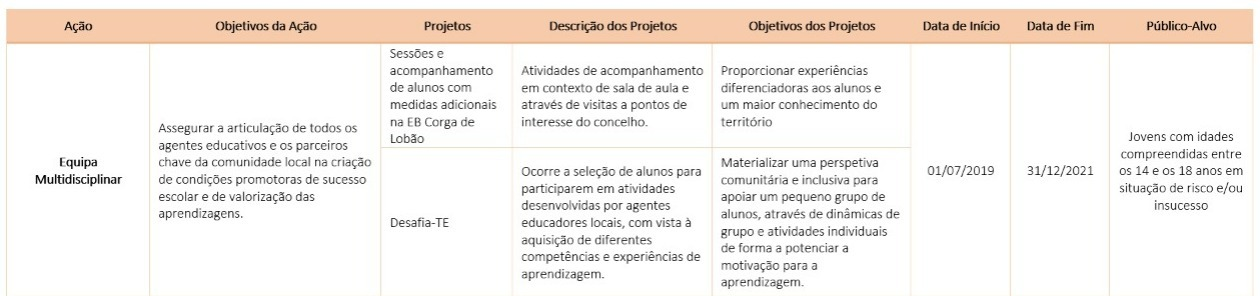
\includegraphics{C:/Users/julio/Documents/bookPoat/imagensRelatorio/figura15.jpg}
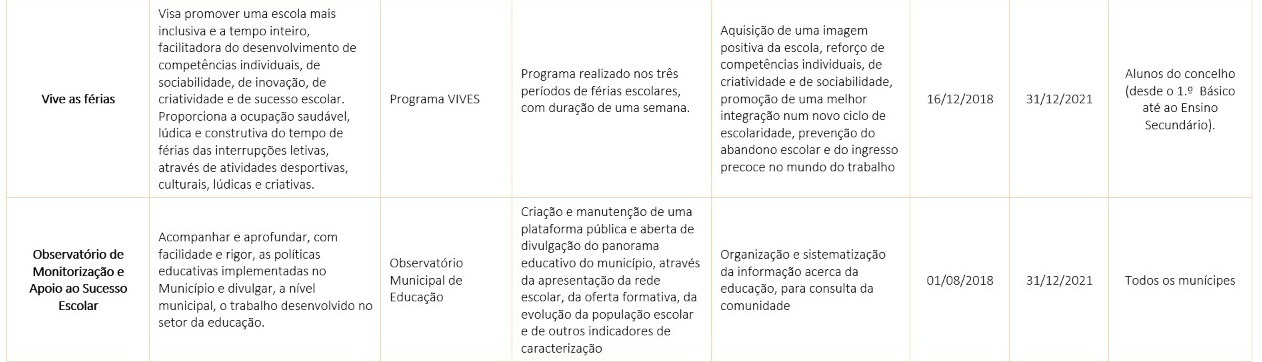
\includegraphics{C:/Users/julio/Documents/bookPoat/imagensRelatorio/figura16.jpg}
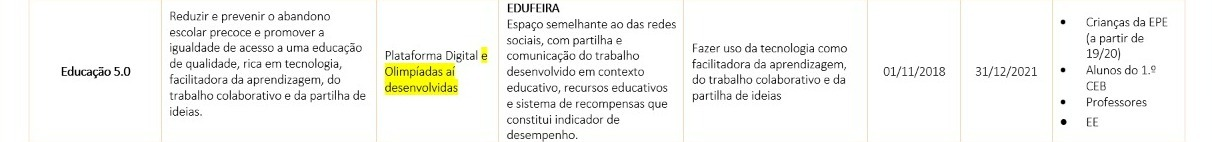
\includegraphics{C:/Users/julio/Documents/bookPoat/imagensRelatorio/figura17.jpg}
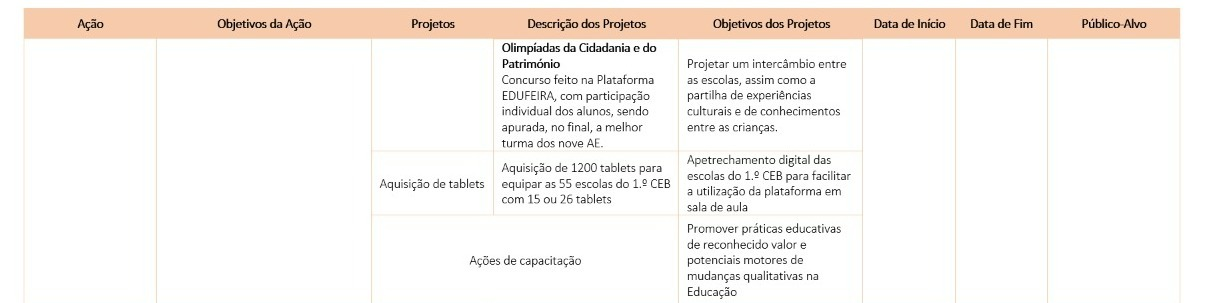
\includegraphics{C:/Users/julio/Documents/bookPoat/imagensRelatorio/figura18.jpg}
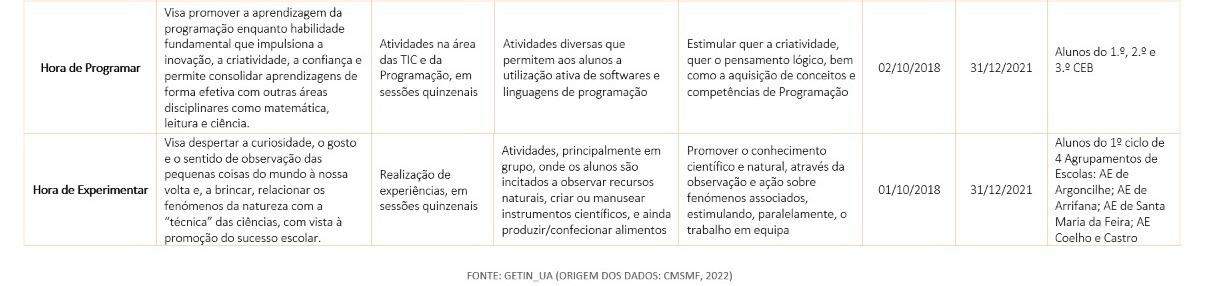
\includegraphics{C:/Users/julio/Documents/bookPoat/imagensRelatorio/figura19.jpg}

\hypertarget{auxe7uxe3o-1---equipa-multidisciplinar}{%
\subsection{\texorpdfstring{\textbf{Ação 1 - Equipa Multidisciplinar}}{Ação 1 - Equipa Multidisciplinar}}\label{auxe7uxe3o-1---equipa-multidisciplinar}}

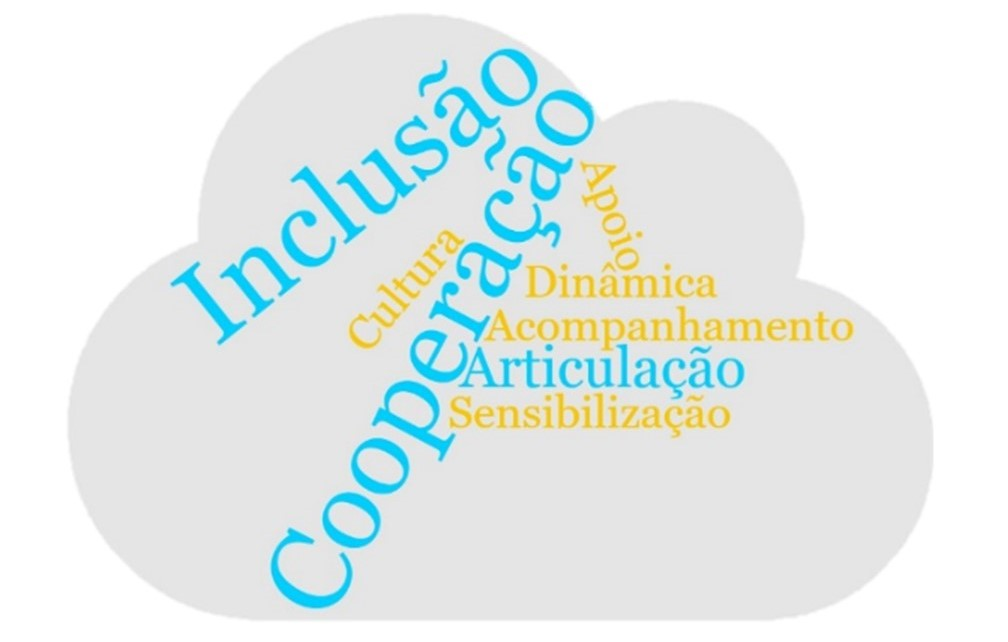
\includegraphics{C:/Users/julio/Documents/bookPoat/imagensRelatorio/figura20.jpg}

Foram desenvolvidos dois projetos: Sessões de acompanhamento de alunos com medidas adicionais na EB Corga de Lobão e o Desafia-te. O primeiro projeto consiste em sessões quinzenais de orientação e suporte destes alunos, envolvendo atividades realizadas tanto em contexto escolar como no exterior. Tendo por base esta definição, realizaram-se atividades na área do desporto, da saúde e da cultura, como por exemplo a construção de um peddy-paper em colaboração com os professores e as visitas ao Zoo de Lourosa e ao Castelo de Santa Maria da Feira.
O Projeto Desafia-te conta com a colaboração dos agrupamentos de escolas do município e com diversos parceiros locais para a realização de sessões em locais diferentes todas as semanas. O processo de seleção para o Desafia-te inclui sessões de divulgação em cada sede de agrupamento, seguidas de inscrições e entrevistas individuais, sendo que todos os anos o grupo de aluno selecionados é alterado. Assim, este projeto pretende proporcionar experiências diferentes de cariz desportivo, cultural, cívico, entre outras, aos selecionados de forma a transmitir uma visão comunitária e inclusiva.

\hypertarget{auxe7uxe3o-2-vive-as-fuxe9rias}{%
\subsection{\texorpdfstring{\textbf{Ação 2 -- Vive as Férias}}{Ação 2 -- Vive as Férias}}\label{auxe7uxe3o-2-vive-as-fuxe9rias}}

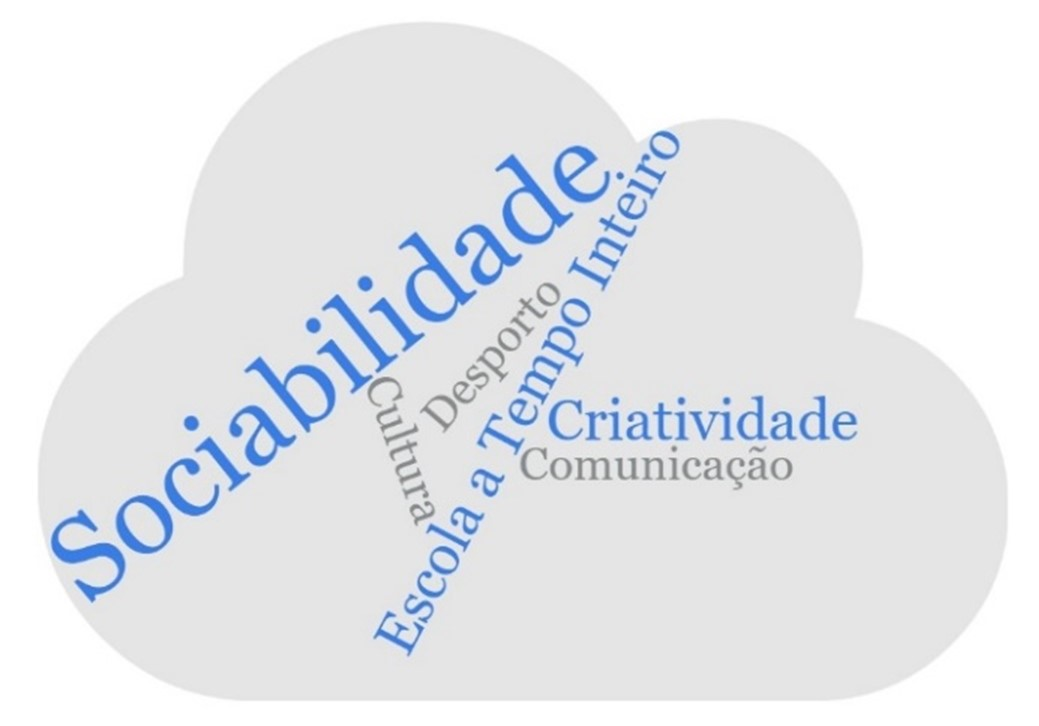
\includegraphics{C:/Users/julio/Documents/bookPoat/imagensRelatorio/figura21.jpg}

Os programas VIVES ocorrem nos três períodos de férias letivas (na Páscoa, Verão e Natal) e têm duração de uma semana para cada grupo de alunos inscritos. Durante esta semana são realizadas atividades, principalmente nas áreas desportiva e cultural, que promovem a criatividade e a inovação, bem como o foco no desenvolvimento de competências individuais e de convivência. As planificações das atividades têm em consideração as idades e as particularidades de cada grupo de alunos.

\hypertarget{auxe7uxe3o-3-observatuxf3rio-de-monitorizauxe7uxe3o-e-apoio-ao-sucesso-escolar}{%
\subsection{\texorpdfstring{\textbf{Ação 3 -- Observatório de monitorização e apoio ao sucesso escolar}}{Ação 3 -- Observatório de monitorização e apoio ao sucesso escolar}}\label{auxe7uxe3o-3-observatuxf3rio-de-monitorizauxe7uxe3o-e-apoio-ao-sucesso-escolar}}

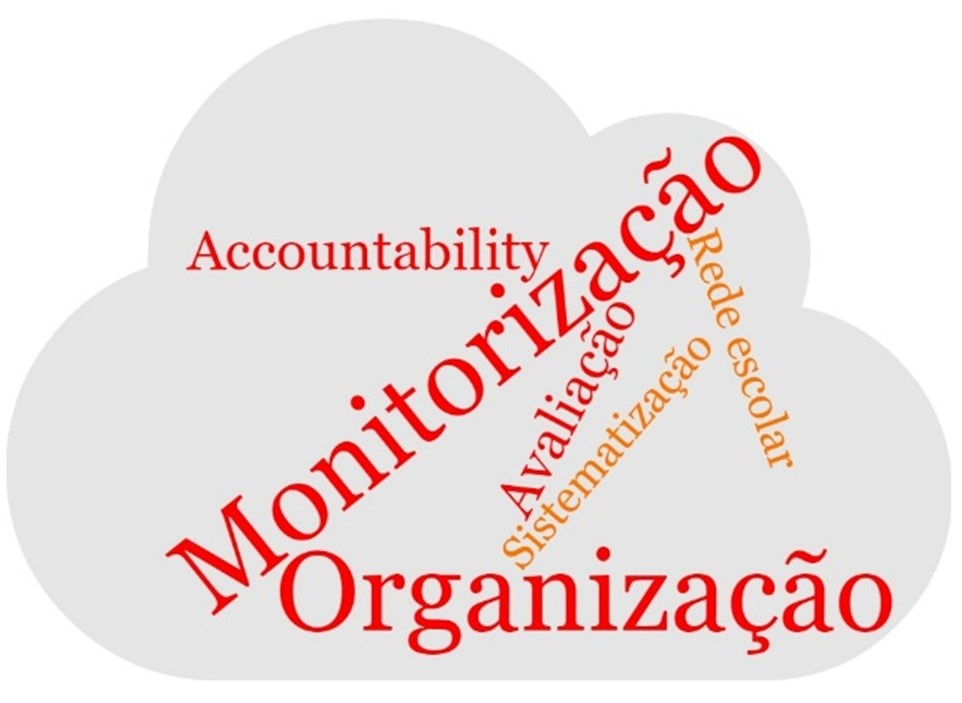
\includegraphics{C:/Users/julio/Documents/bookPoat/imagensRelatorio/figura22.jpg}

O Observatório de Monitorização e Apoio ao Sucesso Escolar tinha como pretensões o acompanhamento das políticas educativas implementadas, a monitorização dos indicadores de níveis de sucesso e a sua correlação com os dados socioeconómicos da população. A construção e atualização permanente desta ferramenta serviriam tanto os decisores políticos no âmbito do planeamento municipal da educação, como a comunidade educativa e qualquer cidadão que aceda aos painéis públicos da plataforma. Uma adicional mais-valia do Observatório residiria na integração na integração do sistema de informação de apoio ao sistema educativo, assim cruzando indicadores. Em última análise, este projeto permitiria o reforço da tomada de decisão com base em evidências, assim como uma maior transparência e accountability.

\hypertarget{auxe7uxe3o-4-educauxe7uxe3o-5.0}{%
\subsection{\texorpdfstring{\textbf{Ação 4 -- Educação 5.0 }}{Ação 4 -- Educação 5.0 }}\label{auxe7uxe3o-4-educauxe7uxe3o-5.0}}

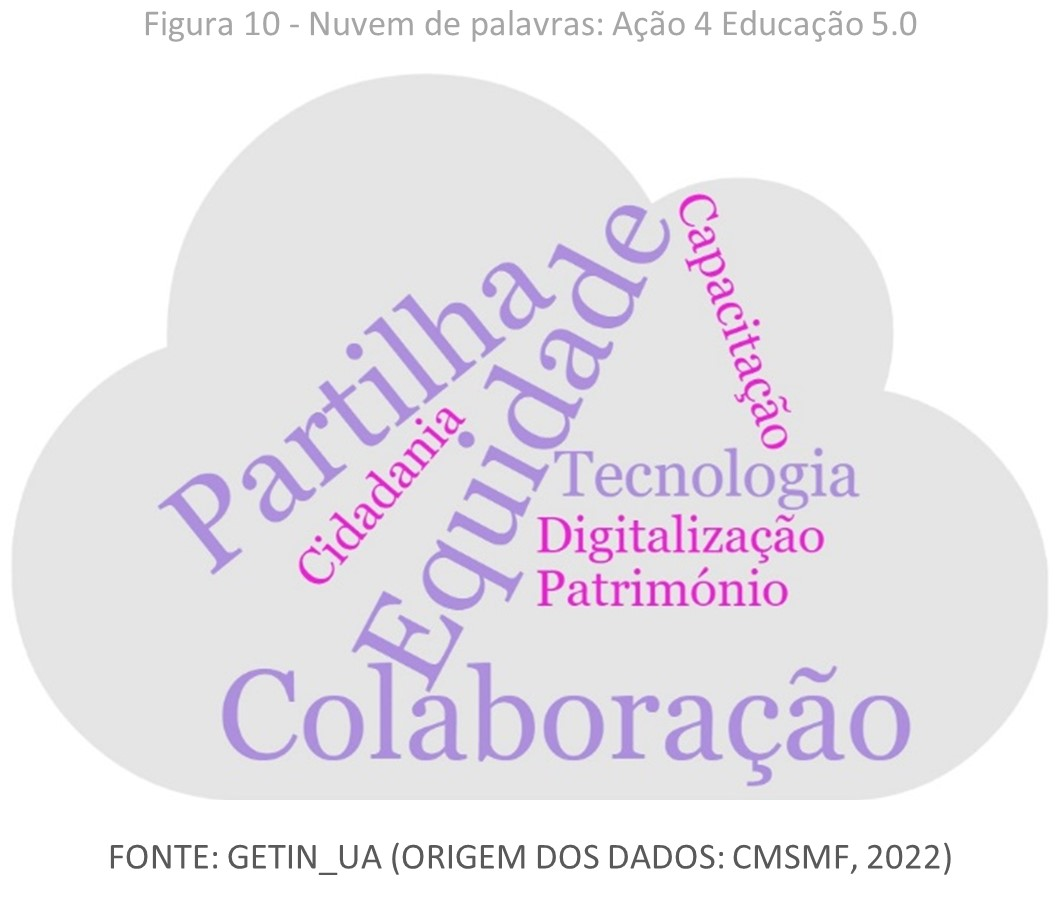
\includegraphics{C:/Users/julio/Documents/bookPoat/imagensRelatorio/figura23.jpg}

Esta ação desenvolveu três projetos: a plataforma digital, aquisição de tablets e ações de capacitação. A plataforma Edufeira destina-se aos alunos do 1º CEB, professores e encarregados de educação e surge como um elemento facilitador de aprendizagem e de partilha de conhecimento, de forma a promover o trabalho colaborativo. Os conteúdos partilhados abrangem temáticas acerca do património de Santa Maria da Feira, da cidadania, apoio ao estudo e atividades/desafios para fazer em família. Além destes conteúdos, nos anos letivos 2019/20 e 2020/21, realizou-se o concurso ``Olimpíadas do Património'' para alunos de 3º e 4º ano, onde cada aluno teve a oportunidade de participar individualmente, sendo apurada a melhor turma. Da 1ª fase resultaram nove turmas vencedoras, uma por cada agrupamento de escolas. Na fase final, as turmas apuradas competiram entre si e escolheu-se a vencedora consoante a pontuação adquirida.

Associado a este projeto, o município adquiriu cerca de 1200 tablets para equipar as 55 escolas de 1º ciclo, de modo a contribuir para a utilização da plataforma em contexto de sala de aula. As ações de capacitação têm como objetivo divulgar e informar os participantes acerca de práticas educativas promotoras de mudança. Alguns exemplos de ações de capacitação desenvolvidas no âmbito da ação Educação 5.0 são a Oficina de Oficina de Formação Professores e as Jornadas da Educação.

\hypertarget{auxe7uxe3o-5-hora-de-programar}{%
\subsection{\texorpdfstring{\textbf{Ação 5 -- Hora de Programar}}{Ação 5 -- Hora de Programar}}\label{auxe7uxe3o-5-hora-de-programar}}

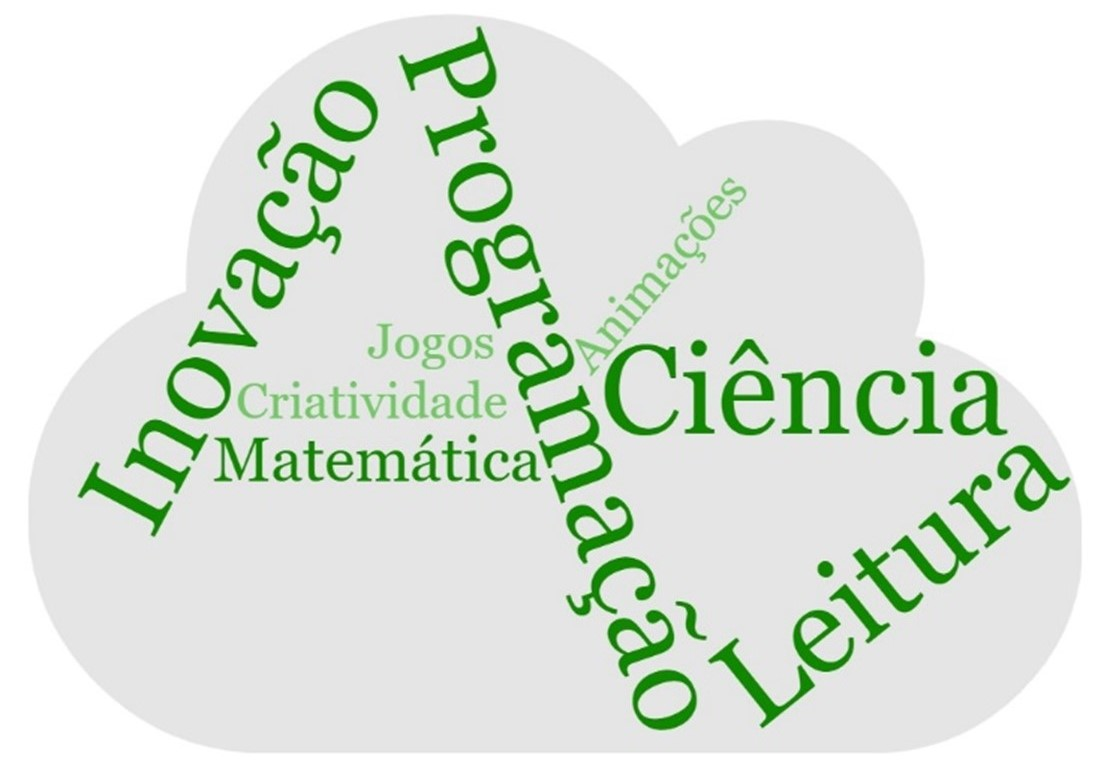
\includegraphics{C:/Users/julio/Documents/bookPoat/imagensRelatorio/figura24.jpg}

No âmbito da ação Hora de Programar foram realizadas sessões quinzenais junto dos alunos de 1º, 2º e 3º CEB com o objetivo de desenvolver competências na área da tecnologia e da programação com o apoio dos professores. A realização de trabalhos escolares nestas sessões promoveu o trabalho em grupo e incentivou o relacionamento entre os alunos. Para além das sessões em contexto de escolar, alguns dos alunos participaram no evento Robô Oeste e no Concurso nacional de programação ``A Criar com Scratch!''.

\hypertarget{auxe7uxe3o-6-hora-de-experimentar}{%
\subsection{\texorpdfstring{\textbf{Ação 6 -- Hora de Experimentar }}{Ação 6 -- Hora de Experimentar }}\label{auxe7uxe3o-6-hora-de-experimentar}}

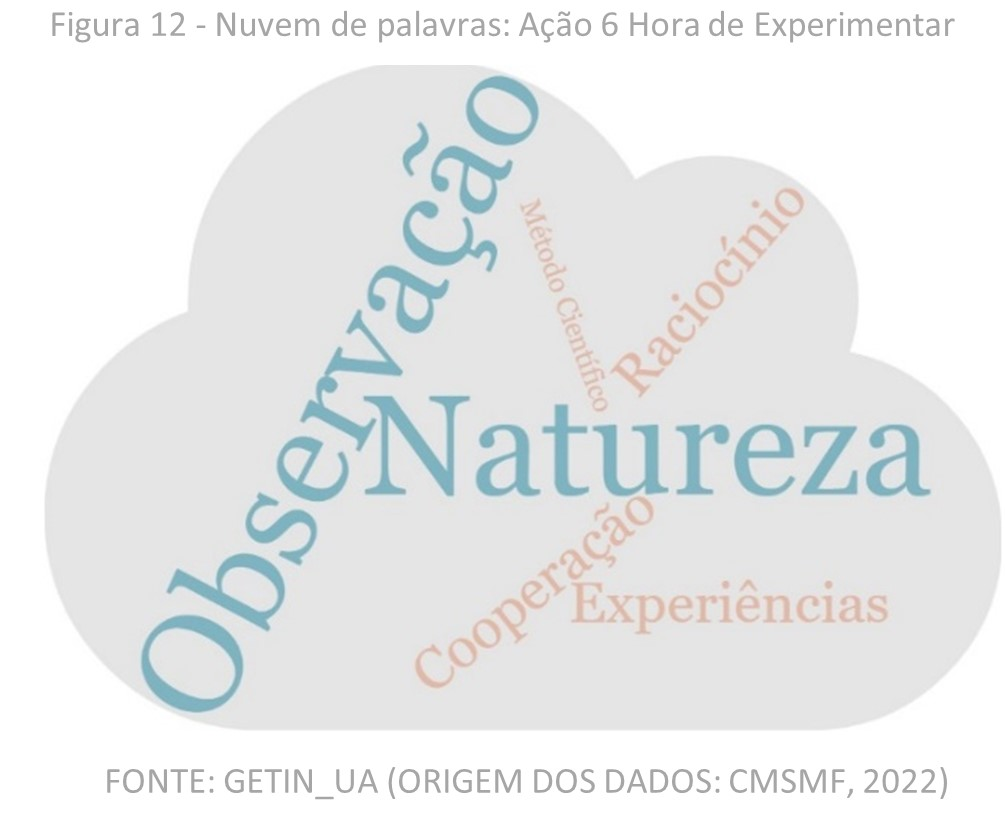
\includegraphics{C:/Users/julio/Documents/bookPoat/imagensRelatorio/figura25.jpg}

A ação Hora de Experimentar foi realizada em quatro agrupamentos do município: Argoncilhe, Arrifana, Santa Maria da Feira e Coelho e Castro. Estes agrupamentos apostaram nas ciências experimentais e desenvolveram sessões quinzenais, onde os alunos têm espaço para fazer experiência científicas e explorar novos desafios. Esta ação promove o raciocínio e a cooperação entre os alunos, fazendo com que estes adquiram novas competências na área da ciência.

\hypertarget{indicadores-de-resultado-e-realizauxe7uxe3o-da-operauxe7uxe3o-cofinanciada}{%
\section{Indicadores de resultado e realização da operação cofinanciada}\label{indicadores-de-resultado-e-realizauxe7uxe3o-da-operauxe7uxe3o-cofinanciada}}

Partilha-se do entendimento avançado pelo relatório de Avaliação do Contributo do PT2020 para a Promoção do Sucesso Educativo, Redução do Abandono Escolar Precoce e Empregabilidade dos jovens, uma vez que não é possível

\begin{quote}
``estabelecer uma relação direta entre os projetos PIICIE e a evolução das taxas de retenção/desistência (pois o território é beneficiário de um conjunto muito mais lato de medidas que podem fazer a diferença)'' (IESE et al., 2021, p.~81)
\end{quote}

Este \emph{caveat} não deve, no entanto, impedir uma análise dos indicadores, designadamente das taxas de retenção e desistência e das taxas de níveis negativos no território em estudo, indicadores contratualizados pela entidade beneficiária. Por outro lado, a leitura dos resultados deve, ainda, estar consciente da conjuntura crítica pandémica, contemporânea de parte do período de análise.

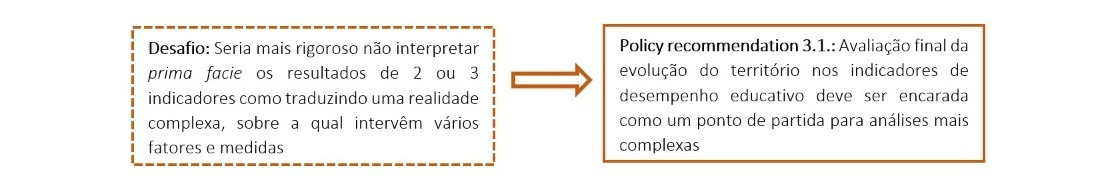
\includegraphics{C:/Users/julio/Documents/bookPoat/imagensRelatorio/figura26.jpg}

Alunos envolvidos nas atividades, por nível de ensino
Meta contratualizada Resultados
4 200 19 891
COMPLEMENTAR COM GRÁFICO OU DASH, POR NÍVEL DE ENSINO

Medidas de cada operação implementadas
Meta contratualizada Resultados
\textgreater80\% Entende-se que a meta foi cumprida

O relatório final do PIICIE Edufeira refere que ``Todas as ações foram executadas, até em período de suspensão das atividades letivas e não letivas presencias, decorrentes da pandemia COVID-19, com exceção de algumas das atividades da ação 2 -- Vive as Férias''.

CONFIRMAR SE CANDIDATURA APRESENTAVA N.º DE MEDIDAS E CONFRONTAR COM O EXECUTADO

Municípios envolvidos na operação
Meta contratualizada Resultados
1 1

Agrupamentos abrangidos
Meta contratualizada Resultados
100\% 100\% (9/9 AE abrangidos)

Redução da taxa de alunos com níveis negativos
Meta contratualizada Resultados\\
\textgreater10\% 2.º CEB: -53\% CONFIRMAR
3.º CEB: -46\% CONFIRMAR
COMPLEMENTAR COM GRÁFICO OU DASH

Redução da taxa de retenção e desistência
Meta contratualizada Resultados
\textgreater25\% 1.º CEB: -44\% CONFIRMAR
2.º CEB: -64\% CONFIRMAR
3.º CEB: -74\% CONFIRMAR
Ensino Secundário: -42\% CONFIRMAR
COMPLEMENTAR COM GRÁFICO OU DASH

\textbf{Grau de satisfação}

Recorrendo a questionários difundidos nos anos letivos 2019/20 e 2020/21, bem como a pareceres solicitados aos AE aquando do término do projeto, a entidade beneficiária concluiu que a meta contratualizada de 90\% foi atingida (REF RELAT SMF). De uma forma geral, os agrupamentos de escolas salientam a importância que o PIICIE teve nos processos de aprendizagem e colaboração para o combate ao insucesso escolar. Destaca-se a necessidade de dar continuidade a vários projetos desenvolvidos e o alargamento destes para todos os alunos, uma vez que produziram experiências inovadoras e úteis no percurso escolar destes, considerando-os um benefício para o município de Santa Maria da Feira. Para além dos agrupamentos, a Fapfeira evidenciou que, apesar dos constrangimentos causados pela pandemia COVID-19, a implementação dos projetos ocorreu de forma positiva, cumprindo as metas propostas. Foi aconselhado, por parte da associação, investir numa maior divulgação das atividades desenvolvidas de forma a informar o maior número de pessoas e aumentar a adesão aos projetos.

\hypertarget{indicadores-especuxedficos-de-caracterizauxe7uxe3o-das-auxe7uxf5es}{%
\section{Indicadores específicos de caracterização das ações}\label{indicadores-especuxedficos-de-caracterizauxe7uxe3o-das-auxe7uxf5es}}

Importa complexificar os indicadores de realização das ações, pelo que os indicadores específicos pretendem cumprir este papel. Assim, alguns dos indicadores são comuns a todas as ações , como é caso dos parceiros envolvidos na formulação e/ou na elaboração e o número total de participantes que

\hypertarget{impacto-da-pandemia-covid-19-na-execuuxe7uxe3o-das-atividades-e-projetos-programados}{%
\chapter{\texorpdfstring{\textbf{Impacto da pandemia Covid-19 na execução das atividades e projetos programados}}{Impacto da pandemia Covid-19 na execução das atividades e projetos programados}}\label{impacto-da-pandemia-covid-19-na-execuuxe7uxe3o-das-atividades-e-projetos-programados}}

A pandemia Covid-19 causou um impacto enorme no sistema educativo, começando pelo ensino à distância e a emergência em fazer adaptações rápidas para dar continuidade ao ensino. Assim, os projetos e as atividades de cada uma das ações tiveram de sofrer alterações inevitáveis.\\
No projeto Desafia-TE, integrado na ação Equipa Multidisciplinar, ocorrem algumas mudanças para que fosse possível continuar a apoiar os jovens selecionados à distância. A partir do mês de março de 2020, foi criado o programa ``Desafia-TE em casa'' que se concretizou através de seis sessões online no 1º período e, desta forma, os desafios do projeto foram cumpridos apesar dos imprevistos. Já o projeto com os alunos abrangidos por medidas adicionais da EB Corga de Lobão manteve-se como planeado, sendo que estes continuaram a ter as sessões presencialmente ainda que a escola estivesse encerrada devido ao confinamento imposto pela pandemia.\\
Em 2020 e 2021, não foi possível concretizar o programa Vives na interrupção letiva da Páscoa. Os programas Vives do Natal realizaram-se, porém houve uma limitação quanto ao número de participantes.\\
No âmbito da ação Educação 5.0 ocorrem iniciativas orientadas para o próprio contexto pandémico como por exemplo, o workshop ``A importância de atividade plásticas e lúdicas em tempos de quarentena'' realizado online.\\
Nas ações da Hora de Programar e da Hora de Experimentar, criou-se um canal no Youtube utilizado para disponibilizar a realização das atividades aos alunos, bem como a utilização da plataforma EDUFEIRA para o mesmo fim. Para além disso, foram fornecidas orientações das atividades para os alunos que por algum motivo não tinham acesso aos conteúdos.

\hypertarget{policy-recommendations}{%
\chapter{Policy recommendations}\label{policy-recommendations}}

Enquadrada pelo Método Aberto de Coordenação, a ação europeia na Educação passa, em larga medida, pela difusão de recomendações. Argumentamos que estas recomendações podem ser mais aprofundadas e detalhadas, designadamente no rescaldo de projetos de avaliação como o presente. Nesta linha, avança-se com recomendações que não se circunscrevem ao território e ao PIICIE de Santa Maria da Feira, ainda que partam deste, das oportunidades e desafios identificados.
Olhando para a proposta do Programa Demografia, Qualificações e Inclusão (atualmente em consulta pública), enquadrado pelo Portugal 2030, confirma-se a manutenção da centralidade das qualificações como aposta estruturante, uma vez que ``o baixo nível de qualificações de uma grande fatia da população continua a ser uma das maiores fragilidades estruturais'' (Portugal 2030, 2022). Assim, assume-se que as recomendações que se seguem podem ser mobilizadas para o sistema de monitorização e avaliação das políticas cofinanciadas de promoção do sucesso escolar, enquadrados pelo quadro 2021-2027.

\hypertarget{recomendauxe7uxf5es-sobre-o-combate-ao-insucesso-escolar}{%
\section{Recomendações sobre o combate ao insucesso escolar}\label{recomendauxe7uxf5es-sobre-o-combate-ao-insucesso-escolar}}

Footnotes are put inside the square brackets after a caret \texttt{\^{}{[}{]}}. Like this one \footnote{This is a footnote.}.

\hypertarget{recomendauxe7uxf5es-metodoluxf3gicas-para-os-programas-de-combate-ao-insucesso-escolar-cofinanciados-no-quadro-2021-2027}{%
\section{Recomendações (metodológicas) para os programas de combate ao insucesso escolar cofinanciados no quadro 2021-2027}\label{recomendauxe7uxf5es-metodoluxf3gicas-para-os-programas-de-combate-ao-insucesso-escolar-cofinanciados-no-quadro-2021-2027}}

Avaliação ex-ante
PR1.1. Atualização do leque de indicadores de desempenho educativo, também designados por `Indicadores de resultado' nos Avisos do QFP 2014-20, de modo a incluir os indicadores de equidade que ganharam força na governação educativa nos últimos anos
Aquando da formulação dos PIICIE e dos primeiros avisos (2016), os indicadores de equidade ainda não haviam sido formulados. Porém, estes impuseram-se recentemente como aqueles mais apropriados para medir o sucesso escolar (DGEEC, 2022a; POCH, 2021). Devem, assim, ser integrados os seguintes indicadores:
• Conclusão no tempo esperado;
• Percursos diretos de sucesso;
• Indicador de equidade, que mede os níveis de sucesso educativo dos alunos de condições socioeconómicas mais frágeis.

PR1.2. Consolidação do papel e posicionamento dos Municípios e das CIM como intermediários entre os órgãos de administração das escolas e as entidades de governo nacionais, designadamente no que diz respeito às estatísticas educativas
Os Municípios e CIM não serão bem-sucedidos, nem rigorosos, na formulação de estratégias educativas se não tiverem conhecimento atualizado sobre as suas realidades. Assim, fazendo uso da interoperabilidade de sistemas (e da crescente difusão de Observatórios Municipais de Educação), a candidatura aos programas de combate ao insucesso deve partir de um diagnóstico de desempenho educativo atualizado e pertinente, que permita identificar aspetos críticos da realidade educativa do território. Os Observatórios deverão ser úteis para lá do diagnóstico, adicionalmente entendidos como essenciais na recolha e sistematização de informação para a monitorização dos programas.
Compreende-se que a DGEEC seja a gatekeeper das estatísticas educativas no contexto português, mas, perante um crescente contexto de descentralização de competências, não é irrazoável ambicionar um papel mais ativo das entidades subnacionais na organização e divulgação daquelas.

PR1.3. Promoção de incentivos para a construção de metas e objetivos territorializados, que capturem e acompanhem a realidade socioeducativa abrangida pela ação.
Os territórios são intrinsecamente diversos, pelo que se argumenta pela necessidade de formular indicadores em coerência com o diagnóstico previamente elaborado. Pelas suas especificidades, estes indicadores, tão contextuais quanto possível, não podem constar nos editais, daí que deva, ao invés, ser criada a estrutura de incentivos adequada. À obrigatoriedade da elaboração do diagnóstico socioeducativo deve seguir-se uma consequente bateria de indicadores específicos, construída pela entidade beneficiária.
Para qualquer um dos indicadores, devem ser contratualizados resultados esperados, assim como lançadas as bases para a recolha de dados longitudinais, sobre os participantes envolvidos, que facilitem a elaboração de avaliações de impacto. Estes últimos poderão contemplar, por exemplo, níveis de aproveitamento e percurso escolar dos alunos participantes. Ainda que aparente ser um exercício de elevada abstração, representa uma etapa fulcral para o futuro confronto do projetado e do alcançado, de modo a acompanhar e aferir o sucesso da operação.

PR1.4. Robustecimento do diálogo entre a estratégia educativa do território e o PIICIE a implementar
Deve ser evitada a multiplicação de estratégias difusas, assegurando a convergência dos programas de combate ao insucesso com as estratégias escolares, municipais e intermunicipais implementadas que, por sua vez, deverão intimamente relacionadas com os desafios educativos territoriais. Apenas deste modo será possível investir numa política educativa robusta, integrada e de continuidade.

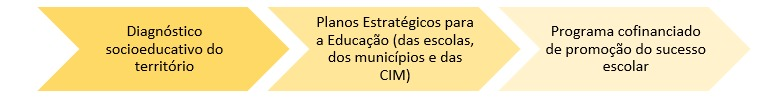
\includegraphics{C:/Users/julio/Documents/bookPoat/imagensRelatorio/img13.jpeg}

Recomenda-se, assim, o preenchimento, em sede de candidatura, de uma grelha similar à seguinte, explicitando este desejado diálogo.

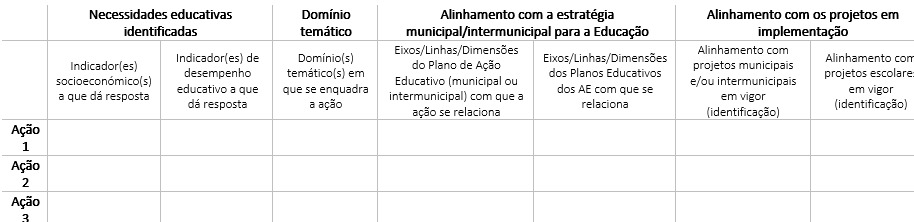
\includegraphics{C:/Users/julio/Documents/bookPoat/imagensRelatorio/img14.jpeg}

PR1.5. Garantia de condições de gestão e administração das entidades beneficiárias, de forma a aumentar a probabilidade de sucesso na implementação da operação
O sucesso do plano de promoção do sucesso depende, em larga medida, dos Recursos Humanos mobilizados para a sua implementação e acompanhamento. Sendo estes planos tão dependentes da interação interinstitucional entre atores, é crucial que estes apostem nos momentos de contacto e difusão. Esta necessidade torna-se mais premente em planos dinamizados por CIM, onde a rede é mais extensa e de mais exigente articulação.\\
Assim, será relevante definir e monitorizar, quantitativamente:
• Técnicos Superiores envolvidos no acompanhamento do plano;
• Reuniões internas sobre o plano;
• Reuniões da entidade beneficiária com entidades parceiras;
• Instrumentos de avaliação;
• Sessões abertas à comunidade educativa para divulgação do plano.

\textbf{Monitorização}

PR2.1. Acompanhamento e avaliação periódica da evolução do território nos indicadores de desempenho educativo e nos indicadores de realização das ações
Os relatórios anuais que as entidades beneficiárias remetem à autoridade de gestão, indicando as ações desenvolvidas durante esse período, deverão compreender, igualmente, a evolução do território nos indicadores de desempenho educativo. Sendo um dos desafios, na avaliação de políticas educativas, o desfasamento temporal na publicação de estatísticas educativas, torna-se ainda mais urgente a formalização de maiores competências das entidades subnacionais neste sentido.
O acompanhamento da evolução dos indicadores de desempenho educativo possibilita a identificação de desafios ao longo da implementação do PIICIE, conduzindo a pequenos ajustes do plano para fazer face àqueles. Não sendo desejáveis desvios significativos face ao estabelecido na memória descritiva do projeto, tais ajustes devem ser formulados com parcimónia.
Paralelamente, importa também encetar regularmente uma avaliação da execução face à previsão no que concerne os indicadores de realização de cada uma das ações, olhando para:
• Alunos participantes;
• Encarregados de Educação participantes;
• Docentes envolvidos;
• Parcerias criadas;
• Atividades realizadas.
Os indicadores propostos na PR1.5. devem também ser alvo desta monitorização anual.

Avaliação ex-post
PR3.1. Avaliação final da evolução do território nos indicadores de desempenho educativo deve ser encarada como um ponto de partida para análises mais complexas
Naturalmente, e à semelhança do realizado nesta primeira geração de PIICIE, as entidades devem prestar contas, no final da execução do projeto, sobre a evolução do território face às metas contratualizadas, incidentes sobre o desempenho educativo e a realização das ações.
Olhar para os indicadores de desempenho educativo não traduzirá de forma completa e fiel o efeito dos PIICIE, uma vez que certamente não serão a única medida de promoção do sucesso. A própria terminologia ``indicadores de resultado'', adotada no quadro 2014-20, é enganadora. Estes indicadores são, porém, essenciais para análises de correlação e causalidade mais sofisticadas.
Adicionalmente, é ideal que tenha sido colocada em ação, desde o arranque do projeto, a matriz de recolha de dados longitudinais mencionada na PR1.3.

PR3.2. Disseminação dos resultados através de eventos públicos e da comunicação institucional
Entende-se que os programas cofinanciados de promoção do sucesso escolar não podem permanecer exclusivamente na esfera das entidades beneficiárias e parceiras. Deve, por isso, ser encetado um esforço de divulgação das ações e dos respetivos resultados junto de toda a comunidade educativa do território em questão, assim promovendo a visibilidade do cofinanciamento europeu na área da Educação.

Reference items in your bibliography file(s) using \texttt{@key}.

For example, we are using the \textbf{bookdown} package \citep{R-bookdown} (check out the last code chunk in index.Rmd to see how this citation key was added) in this sample book, which was built on top of R Markdown and \textbf{knitr} \citep{xie2015} (this citation was added manually in an external file book.bib).
Note that the \texttt{.bib} files need to be listed in the index.Rmd with the YAML \texttt{bibliography} key.

The RStudio Visual Markdown Editor can also make it easier to insert citations: \url{https://rstudio.github.io/visual-markdown-editing/\#/citations}

\hypertarget{recomendauxe7uxf5es-sobre-a-atuauxe7uxe3o-das-comunidades-intermunicipais}{%
\section{Recomendações sobre a atuação das Comunidades Intermunicipais}\label{recomendauxe7uxf5es-sobre-a-atuauxe7uxe3o-das-comunidades-intermunicipais}}

Antecipa-se que as Comunidades Intermunicipais venham a reforçar a sua atuação no combate ao insucesso escolar. O POR Norte para o período de programação 2021-2027 já se encontra a preparar os Planos Intermunicipais de Promoção do Sucesso Escolar (PIPSE), sucessores dos PIICIE (PT 2 PT Índic\textgreater, n.d.). ERRO REF Tal alteração torna as CIM e a AMP as únicas entidades beneficiárias destas políticas cofinanciadas, numa transferência que aparenta reforçar as suas responsabilidades. Este caminho deve, no entanto, ser trilhado com a consciência dos desafios subjacentes. Alguns destes foram já mencionados nas orientações associadas a cada fase de avaliação dos programas de combate ao insucesso, mas importa sistematizá-los, sendo vários deles associados a problemas de ação coletiva e de delegação/externalização . Garrone et al.~(2012) ou Allers e de Greef (2017) concluem que a cooperação intermunicipal pode levar a perdas de eficiência.

\textbf{REFERÊNCIAS BIBLIOGRÁFICAS E ELETRÓNICAS}
Presidência do Conselho de Ministros. (2018). ``Decreto-Lei 54/2018''. Diário da República 1ª série, 129 (julho): 2918 -- 2928. \url{https://data.dre.pt/eli/dec-lei/54/2018/07/06/p/dre/pt/html}
\# Policy recommendations

Enquadrada pelo Método Aberto de Coordenação, a ação europeia na Educação passa, em larga medida, pela difusão de recomendações. Argumentamos que estas recomendações podem ser mais aprofundadas e detalhadas, designadamente no rescaldo de projetos de avaliação como o presente. Nesta linha, avança-se com recomendações que não se circunscrevem ao território e ao PIICIE de Santa Maria da Feira, ainda que partam deste, das oportunidades e desafios identificados.
Olhando para a proposta do Programa Demografia, Qualificações e Inclusão (atualmente em consulta pública), enquadrado pelo Portugal 2030, confirma-se a manutenção da centralidade das qualificações como aposta estruturante, uma vez que ``o baixo nível de qualificações de uma grande fatia da população continua a ser uma das maiores fragilidades estruturais'' (Portugal 2030, 2022). Assim, assume-se que as recomendações que se seguem podem ser mobilizadas para o sistema de monitorização e avaliação das políticas cofinanciadas de promoção do sucesso escolar, enquadrados pelo quadro 2021-2027.

\hypertarget{recomendauxe7uxf5es-sobre-o-combate-ao-insucesso-escolar-1}{%
\section{Recomendações sobre o combate ao insucesso escolar}\label{recomendauxe7uxf5es-sobre-o-combate-ao-insucesso-escolar-1}}

Footnotes are put inside the square brackets after a caret \texttt{\^{}{[}{]}}. Like this one \footnote{This is a footnote.}.

\hypertarget{recomendauxe7uxf5es-metodoluxf3gicas-para-os-programas-de-combate-ao-insucesso-escolar-cofinanciados-no-quadro-2021-2027-1}{%
\section{Recomendações (metodológicas) para os programas de combate ao insucesso escolar cofinanciados no quadro 2021-2027}\label{recomendauxe7uxf5es-metodoluxf3gicas-para-os-programas-de-combate-ao-insucesso-escolar-cofinanciados-no-quadro-2021-2027-1}}

Avaliação ex-ante
PR1.1. Atualização do leque de indicadores de desempenho educativo, também designados por `Indicadores de resultado' nos Avisos do QFP 2014-20, de modo a incluir os indicadores de equidade que ganharam força na governação educativa nos últimos anos
Aquando da formulação dos PIICIE e dos primeiros avisos (2016), os indicadores de equidade ainda não haviam sido formulados. Porém, estes impuseram-se recentemente como aqueles mais apropriados para medir o sucesso escolar (DGEEC, 2022a; POCH, 2021). Devem, assim, ser integrados os seguintes indicadores:
• Conclusão no tempo esperado;
• Percursos diretos de sucesso;
• Indicador de equidade, que mede os níveis de sucesso educativo dos alunos de condições socioeconómicas mais frágeis.

PR1.2. Consolidação do papel e posicionamento dos Municípios e das CIM como intermediários entre os órgãos de administração das escolas e as entidades de governo nacionais, designadamente no que diz respeito às estatísticas educativas
Os Municípios e CIM não serão bem-sucedidos, nem rigorosos, na formulação de estratégias educativas se não tiverem conhecimento atualizado sobre as suas realidades. Assim, fazendo uso da interoperabilidade de sistemas (e da crescente difusão de Observatórios Municipais de Educação), a candidatura aos programas de combate ao insucesso deve partir de um diagnóstico de desempenho educativo atualizado e pertinente, que permita identificar aspetos críticos da realidade educativa do território. Os Observatórios deverão ser úteis para lá do diagnóstico, adicionalmente entendidos como essenciais na recolha e sistematização de informação para a monitorização dos programas.
Compreende-se que a DGEEC seja a gatekeeper das estatísticas educativas no contexto português, mas, perante um crescente contexto de descentralização de competências, não é irrazoável ambicionar um papel mais ativo das entidades subnacionais na organização e divulgação daquelas.

PR1.3. Promoção de incentivos para a construção de metas e objetivos territorializados, que capturem e acompanhem a realidade socioeducativa abrangida pela ação.
Os territórios são intrinsecamente diversos, pelo que se argumenta pela necessidade de formular indicadores em coerência com o diagnóstico previamente elaborado. Pelas suas especificidades, estes indicadores, tão contextuais quanto possível, não podem constar nos editais, daí que deva, ao invés, ser criada a estrutura de incentivos adequada. À obrigatoriedade da elaboração do diagnóstico socioeducativo deve seguir-se uma consequente bateria de indicadores específicos, construída pela entidade beneficiária.
Para qualquer um dos indicadores, devem ser contratualizados resultados esperados, assim como lançadas as bases para a recolha de dados longitudinais, sobre os participantes envolvidos, que facilitem a elaboração de avaliações de impacto. Estes últimos poderão contemplar, por exemplo, níveis de aproveitamento e percurso escolar dos alunos participantes. Ainda que aparente ser um exercício de elevada abstração, representa uma etapa fulcral para o futuro confronto do projetado e do alcançado, de modo a acompanhar e aferir o sucesso da operação.

PR1.4. Robustecimento do diálogo entre a estratégia educativa do território e o PIICIE a implementar
Deve ser evitada a multiplicação de estratégias difusas, assegurando a convergência dos programas de combate ao insucesso com as estratégias escolares, municipais e intermunicipais implementadas que, por sua vez, deverão intimamente relacionadas com os desafios educativos territoriais. Apenas deste modo será possível investir numa política educativa robusta, integrada e de continuidade.

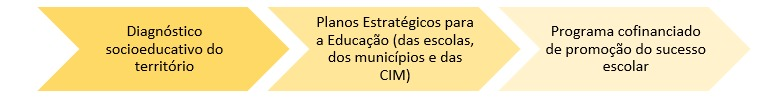
\includegraphics{C:/Users/julio/Documents/bookPoat/imagensRelatorio/img13.jpeg}

Recomenda-se, assim, o preenchimento, em sede de candidatura, de uma grelha similar à seguinte, explicitando este desejado diálogo.

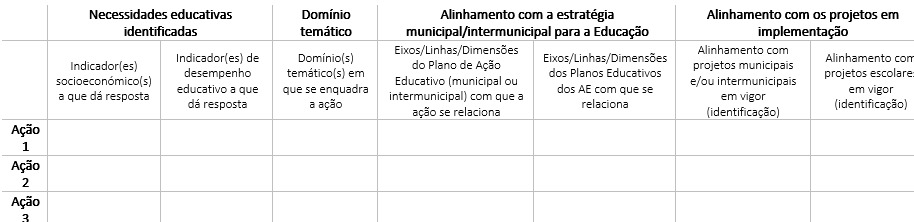
\includegraphics{C:/Users/julio/Documents/bookPoat/imagensRelatorio/img14.jpeg}

PR1.5. Garantia de condições de gestão e administração das entidades beneficiárias, de forma a aumentar a probabilidade de sucesso na implementação da operação
O sucesso do plano de promoção do sucesso depende, em larga medida, dos Recursos Humanos mobilizados para a sua implementação e acompanhamento. Sendo estes planos tão dependentes da interação interinstitucional entre atores, é crucial que estes apostem nos momentos de contacto e difusão. Esta necessidade torna-se mais premente em planos dinamizados por CIM, onde a rede é mais extensa e de mais exigente articulação.\\
Assim, será relevante definir e monitorizar, quantitativamente:
• Técnicos Superiores envolvidos no acompanhamento do plano;
• Reuniões internas sobre o plano;
• Reuniões da entidade beneficiária com entidades parceiras;
• Instrumentos de avaliação;
• Sessões abertas à comunidade educativa para divulgação do plano.

\textbf{Monitorização}

PR2.1. Acompanhamento e avaliação periódica da evolução do território nos indicadores de desempenho educativo e nos indicadores de realização das ações
Os relatórios anuais que as entidades beneficiárias remetem à autoridade de gestão, indicando as ações desenvolvidas durante esse período, deverão compreender, igualmente, a evolução do território nos indicadores de desempenho educativo. Sendo um dos desafios, na avaliação de políticas educativas, o desfasamento temporal na publicação de estatísticas educativas, torna-se ainda mais urgente a formalização de maiores competências das entidades subnacionais neste sentido.
O acompanhamento da evolução dos indicadores de desempenho educativo possibilita a identificação de desafios ao longo da implementação do PIICIE, conduzindo a pequenos ajustes do plano para fazer face àqueles. Não sendo desejáveis desvios significativos face ao estabelecido na memória descritiva do projeto, tais ajustes devem ser formulados com parcimónia.
Paralelamente, importa também encetar regularmente uma avaliação da execução face à previsão no que concerne os indicadores de realização de cada uma das ações, olhando para:
• Alunos participantes;
• Encarregados de Educação participantes;
• Docentes envolvidos;
• Parcerias criadas;
• Atividades realizadas.
Os indicadores propostos na PR1.5. devem também ser alvo desta monitorização anual.

Avaliação ex-post
PR3.1. Avaliação final da evolução do território nos indicadores de desempenho educativo deve ser encarada como um ponto de partida para análises mais complexas
Naturalmente, e à semelhança do realizado nesta primeira geração de PIICIE, as entidades devem prestar contas, no final da execução do projeto, sobre a evolução do território face às metas contratualizadas, incidentes sobre o desempenho educativo e a realização das ações.
Olhar para os indicadores de desempenho educativo não traduzirá de forma completa e fiel o efeito dos PIICIE, uma vez que certamente não serão a única medida de promoção do sucesso. A própria terminologia ``indicadores de resultado'', adotada no quadro 2014-20, é enganadora. Estes indicadores são, porém, essenciais para análises de correlação e causalidade mais sofisticadas.
Adicionalmente, é ideal que tenha sido colocada em ação, desde o arranque do projeto, a matriz de recolha de dados longitudinais mencionada na PR1.3.

PR3.2. Disseminação dos resultados através de eventos públicos e da comunicação institucional
Entende-se que os programas cofinanciados de promoção do sucesso escolar não podem permanecer exclusivamente na esfera das entidades beneficiárias e parceiras. Deve, por isso, ser encetado um esforço de divulgação das ações e dos respetivos resultados junto de toda a comunidade educativa do território em questão, assim promovendo a visibilidade do cofinanciamento europeu na área da Educação.

Reference items in your bibliography file(s) using \texttt{@key}.

For example, we are using the \textbf{bookdown} package \citep{R-bookdown} (check out the last code chunk in index.Rmd to see how this citation key was added) in this sample book, which was built on top of R Markdown and \textbf{knitr} \citep{xie2015} (this citation was added manually in an external file book.bib).
Note that the \texttt{.bib} files need to be listed in the index.Rmd with the YAML \texttt{bibliography} key.

The RStudio Visual Markdown Editor can also make it easier to insert citations: \url{https://rstudio.github.io/visual-markdown-editing/\#/citations}

\hypertarget{recomendauxe7uxf5es-sobre-a-atuauxe7uxe3o-das-comunidades-intermunicipais-1}{%
\section{Recomendações sobre a atuação das Comunidades Intermunicipais}\label{recomendauxe7uxf5es-sobre-a-atuauxe7uxe3o-das-comunidades-intermunicipais-1}}

Antecipa-se que as Comunidades Intermunicipais venham a reforçar a sua atuação no combate ao insucesso escolar. O POR Norte para o período de programação 2021-2027 já se encontra a preparar os Planos Intermunicipais de Promoção do Sucesso Escolar (PIPSE), sucessores dos PIICIE (PT 2 PT Índic\textgreater, n.d.). ERRO REF Tal alteração torna as CIM e a AMP as únicas entidades beneficiárias destas políticas cofinanciadas, numa transferência que aparenta reforçar as suas responsabilidades. Este caminho deve, no entanto, ser trilhado com a consciência dos desafios subjacentes. Alguns destes foram já mencionados nas orientações associadas a cada fase de avaliação dos programas de combate ao insucesso, mas importa sistematizá-los, sendo vários deles associados a problemas de ação coletiva e de delegação/externalização . Garrone et al.~(2012) ou Allers e de Greef (2017) concluem que a cooperação intermunicipal pode levar a perdas de eficiência.

\textbf{REFERÊNCIAS BIBLIOGRÁFICAS E ELETRÓNICAS}
Presidência do Conselho de Ministros. (2018). ``Decreto-Lei 54/2018''. Diário da República 1ª série, 129 (julho): 2918 -- 2928. \url{https://data.dre.pt/eli/dec-lei/54/2018/07/06/p/dre/pt/html}
Câmara Municipal de Santa Maria da Feira. Disponível em: \url{https://cm-feira.pt/}.

Mendeley Cite/Mendeley Reference Manager
Agência para o Desenvolvimento e Coesão. (n.d.). Monitorização - Enquadramento. Retrieved August 23, 2022, from \url{https://www.adcoesao.pt/fundos/portugal-2020/monitorizacao/enquadramento/}
Allers, M. A., \& de Greef, J. A. (2017). Intermunicipal cooperation, public spending and service levels. Local Government Studies, 44(1), 127--150. \url{https://doi.org/10.1080/03003930.2017.1380630}
DGEEC. (2022a). Educação Inclusiva 2020/2021. Apoio à Aprendizagem e à Inclusão, escolas da rede pública do Ministério da Educação.
DGEEC. (2022b). Plano 21\textbar23 Escola+. Segundo relatório de monitorização. \url{http://www.dgeec.mec.pt}
Garrone, P., Grilli, L., \& Rousseau, X. (2012). Local Government Studies Management Discretion and Political Interference in Municipal Enterprises. Evidence from Italian Utilities Management Discretion and Political Interference in Municipal Enterprises. Evidence from Italian Utilities. \url{https://doi.org/10.1080/03003930.2012.726198}
Gaspar de Matos, M., Branquinho, C., Noronha, C., Moraes, B., Santos, O., Carvalho, M., Simões, C., Marques, A., Tomé, G., Guedes, F. B., Cerqueira, A., Francisco, R., \& Gaspar, T. (2022). Observatório de Saúde Psicológica e Bem-Estar: Monitorização e Ação.
IESE, ISCTE, \& PPLL Consult. (2021). Avaliação do Contributo do PT2020 para a Promoção do Sucesso Educativo, Redução do Abandono Escolar Precoce e Empregabilidade dos Jovens. \url{https://doi.org/10.38116/bapi25}
Verdasca, J. (2020). Contributos para o desenvolvimento de um sistema de auto e multirregulação educativa. Revista Portuguesa de Investigação Educacional, n.o Especial, 111--143. \url{https://doi.org/10.34632/investigacaoeducacional.2020.8503}

Mendeley Cite/Mendeley Desktop
Carvalho, M., \& Joana, L. (2020). Uma análise comparada: sistemas inspetivos de alguns países. Revista Lusofona de Educacao, 50(50), 27--41. \url{https://doi.org/10.24140/issn.1645-7250.rle50.02}
CCDR-Norte. (2022). Programa Regional do Norte 2021-2027: Proposta. \url{https://www.ccdr-n.pt/storage/app/media/uploaded-files/po20norte202030versc3a3oconsultapublica.pdf}
Decreto-Lei n.o 21/2019, de 30 de janeiro, do Ministério da Administração Interna, Pub. L. No.~Diário da República n.o 21/2019, Série I (2019).
Decreto-Lei n.o 7/2003, de 15 de janeiro, do Ministério das Cidades, Ordenamento do Território e Ambiente, Pub. L. No.~Diário da República n.o 12/2003, Série I-A (2003).
Decreto-Lei n.o 72/2015, de 11 de maio, da Presidência do Conselho de Ministros, Pub. L. No.~Diário da República n.o 90/2015, Série I (2015).
DGEEC. (2022a). Resultados Escolares: Sucesso e Equidade.
DGEEC. (2022b). Taxa de retenção e desistência (\%), por sexo, nível de ensino, ciclo de estudos e ano de escolaridade - Continente, NUTS II, III e Municípios -- 2003/04 a 2020/21. \url{https://www.dgeec.mec.pt/np4/248/}
DGEEC, DGEstE, \& IGeFE. (2021). Carta Educativa, Guião para Elaboração. \url{https://www.igefe.mec.pt/Files/DownloadDocument/17?csrt=5775597188220950806}
Education Scotland. (2015). How good is our school? (4th edition). www.educationscotland.gov.uk/resources/h/hgios4/
Ehren, M., \& Shackleton, N. (2016). Risk-based school inspections: impact of targeted inspection approaches on Dutch secondary schools. Educational Assessment, Evaluation and Accountability, 299--321. \url{https://doi.org/10.1007/s11092-016-9242-0}
INE. (2021). População residente (N.o) por Local de residência, Sexo e Níveis de ensino; Decenal - INE, Recenseamento da população e habitação - Censos 2021. \url{https://www.ine.pt/xportal/xmain?xpid=INE\&xpgid=ine_indicadores\&indOcorrCod=0011168\&xlang=pt}
Inspeção-Geral da Educação e Ciência (IGEC). (2016). Avaliação Externa das Escolas QUADRO DE REFERÊNCIA PARA A AVALIAÇÃO EXTERNA DAS ESCOLAS. \url{https://www.igec.mec.pt/upload/AEE_2016-2017/AEE_16_17_(1)_Quadro_de_Referencia.pdf}
Inspeção-Geral da Educação e Ciência (IGEC). (2018a). Terceiro Ciclo da Avaliação Externa das Escolas - Âmbito, princípios e objetivos. \url{https://www.igec.mec.pt/upload/AEE3_2018/AEE_3_Amb_princ_objetivos.pdf}
Inspeção-Geral da Educação e Ciência (IGEC). (2018b). Terceiro Ciclo da Avaliação Externa das Escolas - Quadro de referência. \url{https://www.igec.mec.pt/upload/AEE3_2018/AEE_3_Quadro_Ref.pdf}
Ioannidou, A. (2010). Educational monitoring and reporting as governance instruments for evidence-based education policy. International Perspectives on Education and Society, 12, 155--172. \url{https://doi.org/10.1108/S1479-3679(2010)0000012011/FULL/XML}
Mairate, A. (2007). The `added value' of European Union Cohesion policy. Regional Studies, 40(2), 167--177. \url{https://doi.org/10.1080/00343400600600496}
Marques, J. L., Neves, R., Grifo, A., Duarte, J., Malta, J., Sousa, M. P., \& Santos, S. (n.d.). Plano Estratégico Educativo Municipal de Santa Maria da Feira 2022-2030.
Marques, J. L., Wolf, J., Borges, M., \& Batista, P. (2020). Sistemas de apoio à decisão em planeamento: desafios metodológicos e conceptuais. TPU: Território, Planeamento e Urbanismo: Teoria e Prática, 2, 52--79. \url{https://doi.org/10.34624/TPU.V0I2.23720}
Ministério da Educação. (2011). Propostas para um novo ciclo de avaliação externa de escolas, Relatório Final, Grupo de Trabalho para a Avaliação Externa das Escolas 2011. \url{https://www.igec.mec.pt/upload/AEE2_2011/AEE2_GT_2011_RELATORIO_FINAL.pdf}
Ministério da Educação, \& Inspeção-Geral da Educação (IGE). (2010). QUADRO DE REFERÊNCIA PARA A AVALIAÇÃO DE ESCOLAS E AGRUPAMENTOS DE ESCOLAS. \url{https://www.igec.mec.pt/upload/AEE_2011/AEE_10_11_Quadro_Referencia.pdf}
Nóvoa, A. (2013). The Blindness of Europe: New Fabrications in the European Educational Space. SISYPHUS Journal of Education, 1(1), 104--123. \url{http://ec.europa.eu/europe2020/services/faqs/index_en.htm}
Oliveira, P., Clímaco, M., Carravilla, M., Sarrico, C., Azevedo, M., \& Oliveira, J. (2006). Relatório final da actividade do Grupo de Trabalho para Avaliação das Escolas Dezembro 2006. \url{https://www.igec.mec.pt/upload/Relatorios/AEE_06_RELATORIO_GT.pdf}
POCH. (2021). Novo indicador de equidade na educação. \url{https://www.poch.portugal2020.pt/pt-pt/Noticias/Paginas/noticia.aspx?nid=750}
Portugal 2030. (2022). Programa Demografia, Qualificações e Inclusão - Proposta de programa.
Santos, S., Duarte, J. \& Marques, J. L. (2019). Quadro de referência aplicado aos instrumentos de gestão da rede e da política educativa à escala local. Revista de Desarrollo Sustentable, Negocios, Emprendimiento y Educación, 1(1), 1--19.
The Educational Institute of Scotland (EIS). (2019). EDUCATION SCOTLAND INSPECTIONS, General, Advice for members. www.eis.org.uk
XXI GOVERNO - REPÚBLICA PORTUGUESA. (2019, February). Modelo de Avaliação Externa das Escolas -- novo ciclo / Avaliação externa alargada às escolas profissionais privadas e às escolas com contrato de associação/patrocínio. NOTA À COMUNICAÇÃO SOCIAL. \url{https://www.portugal.gov.pt/download-ficheiros/ficheiro.aspx?v=\%3D\%3DBAAAAB\%2BLCAAAAAAABAAzN7Q0AQCs6SFGBAAAAA\%3D\%3D}

\hypertarget{referuxeancias-bibliogruxe1ficas-e-eletruxf3nicas}{%
\chapter*{REFERÊNCIAS BIBLIOGRÁFICAS E ELETRÓNICAS}\label{referuxeancias-bibliogruxe1ficas-e-eletruxf3nicas}}
\addcontentsline{toc}{chapter}{REFERÊNCIAS BIBLIOGRÁFICAS E ELETRÓNICAS}

Presidência do Conselho de Ministros. (2018). ``Decreto-Lei 54/2018''. Diário da República 1ª série, 129 (julho): 2918 -- 2928. \url{https://data.dre.pt/eli/dec-lei/54/2018/07/06/p/dre/pt/html}

Câmara Municipal de Santa Maria da Feira. Disponível em: \url{https://cm-feira.pt/}.

Mendeley Cite/Mendeley Reference Manager

Agência para o Desenvolvimento e Coesão. (n.d.). Monitorização - Enquadramento. Retrieved August 23, 2022, from \url{https://www.adcoesao.pt/fundos/portugal-2020/monitorizacao/enquadramento/}

Allers, M. A., \& de Greef, J. A. (2017). Intermunicipal cooperation, public spending and service levels. Local Government Studies, 44(1), 127--150. \url{https://doi.org/10.1080/03003930.2017.1380630}

DGEEC. (2022a). Educação Inclusiva 2020/2021. Apoio à Aprendizagem e à Inclusão, escolas da rede pública do Ministério da Educação.

DGEEC. (2022b). Plano 21\textbar23 Escola+. Segundo relatório de monitorização. \url{http://www.dgeec.mec.pt}

Garrone, P., Grilli, L., \& Rousseau, X. (2012). Local Government Studies Management Discretion and Political Interference in Municipal Enterprises. Evidence from Italian Utilities Management Discretion and Political Interference in Municipal Enterprises. Evidence from Italian Utilities. \url{https://doi.org/10.1080/03003930.2012.726198}
Gaspar de Matos, M., Branquinho, C., Noronha, C., Moraes, B., Santos, O., Carvalho, M., Simões, C., Marques, A., Tomé, G., Guedes, F. B., Cerqueira, A., Francisco, R., \& Gaspar, T. (2022). Observatório de Saúde Psicológica e Bem-Estar: Monitorização e Ação.
IESE, ISCTE, \& PPLL Consult. (2021). Avaliação do Contributo do PT2020 para a Promoção do Sucesso Educativo, Redução do Abandono Escolar Precoce e Empregabilidade dos Jovens. \url{https://doi.org/10.38116/bapi25}
Verdasca, J. (2020). Contributos para o desenvolvimento de um sistema de auto e multirregulação educativa. Revista Portuguesa de Investigação Educacional, n.o Especial, 111--143. \url{https://doi.org/10.34632/investigacaoeducacional.2020.8503}

Mendeley Cite/Mendeley Desktop
Carvalho, M., \& Joana, L. (2020). Uma análise comparada: sistemas inspetivos de alguns países. Revista Lusofona de Educacao, 50(50), 27--41. \url{https://doi.org/10.24140/issn.1645-7250.rle50.02}
CCDR-Norte. (2022). Programa Regional do Norte 2021-2027: Proposta. \url{https://www.ccdr-n.pt/storage/app/media/uploaded-files/po20norte202030versc3a3oconsultapublica.pdf}
DGEEC. (2022). Resultados Escolares: Sucesso e Equidade.
DGEEC, DGEstE, \& IGeFE. (2021). Carta Educativa, Guião para Elaboração. \url{https://www.igefe.mec.pt/Files/DownloadDocument/17?csrt=5775597188220950806}
Education Scotland. (2015). How good is our school? (4th edition). www.educationscotland.gov.uk/resources/h/hgios4/
Ehren, M., \& Shackleton, N. (2016). Risk-based school inspections: impact of targeted inspection approaches on Dutch secondary schools. Educational Assessment, Evaluation and Accountability, 299--321. \url{https://doi.org/10.1007/s11092-016-9242-0}
Inspeção-Geral da Educação e Ciência (IGEC). (2016). Avaliação Externa das Escolas QUADRO DE REFERÊNCIA PARA A AVALIAÇÃO EXTERNA DAS ESCOLAS. \url{https://www.igec.mec.pt/upload/AEE_2016-2017/AEE_16_17_(1)_Quadro_de_Referencia.pdf}
Inspeção-Geral da Educação e Ciência (IGEC). (2018a). Terceiro Ciclo da Avaliação Externa das Escolas - Âmbito, princípios e objetivos. \url{https://www.igec.mec.pt/upload/AEE3_2018/AEE_3_Amb_princ_objetivos.pdf}
Inspeção-Geral da Educação e Ciência (IGEC). (2018b). Terceiro Ciclo da Avaliação Externa das Escolas - Quadro de referência. \url{https://www.igec.mec.pt/upload/AEE3_2018/AEE_3_Quadro_Ref.pdf}
Ioannidou, A. (2010). Educational monitoring and reporting as governance instruments for evidence-based education policy. International Perspectives on Education and Society, 12, 155--172. \url{https://doi.org/10.1108/S1479-3679(2010)0000012011/FULL/XML}
Marques, J. L., Wolf, J., Borges, M., \& Batista, P. (2020). Sistemas de apoio à decisão em planeamento: desafios metodológicos e conceptuais. TPU: Território, Planeamento e Urbanismo: Teoria e Prática, 2, 52--79. \url{https://doi.org/10.34624/TPU.V0I2.23720}
Ministério da Educação. (2011). Propostas para um novo ciclo de avaliação externa de escolas, Relatório Final, Grupo de Trabalho para a Avaliação Externa das Escolas 2011. \url{https://www.igec.mec.pt/upload/AEE2_2011/AEE2_GT_2011_RELATORIO_FINAL.pdf}
Ministério da Educação, \& Inspeção-Geral da Educação (IGE). (2010). QUADRO DE REFERÊNCIA PARA A AVALIAÇÃO DE ESCOLAS E AGRUPAMENTOS DE ESCOLAS. \url{https://www.igec.mec.pt/upload/AEE_2011/AEE_10_11_Quadro_Referencia.pdf}
Oliveira, P., Clímaco, M., Carravilla, M., Sarrico, C., Azevedo, M., \& Oliveira, J. (2006). Relatório final da actividade do Grupo de Trabalho para Avaliação das Escolas Dezembro 2006. \url{https://www.igec.mec.pt/upload/Relatorios/AEE_06_RELATORIO_GT.pdf}
POCH. (2021). Novo indicador de equidade na educação. \url{https://www.poch.portugal2020.pt/pt-pt/Noticias/Paginas/noticia.aspx?nid=750}
Portugal 2030. (2022). Programa Demografia, Qualificações e Inclusão - Proposta de programa.
Santos, S., Duarte, J. \& Marques, J. L. (2019). Quadro de referência aplicado aos instrumentos de gestão da rede e da política educativa à escala local. Revista de Desarrollo Sustentable, Negocios, Emprendimiento y Educación, 1(1), 1--19.
The Educational Institute of Scotland (EIS). (2019). EDUCATION SCOTLAND INSPECTIONS, General, Advice for members. www.eis.org.uk
XXI GOVERNO - REPÚBLICA PORTUGUESA. (2019, February). Modelo de Avaliação Externa das Escolas -- novo ciclo / Avaliação externa alargada às escolas profissionais privadas e às escolas com contrato de associação/patrocínio. NOTA À COMUNICAÇÃO SOCIAL. \url{https://www.portugal.gov.pt/download-ficheiros/ficheiro.aspx?v=\%3D\%3DBAAAAB\%2BLCAAAAAAABAAzN7Q0AQCs6SFGBAAAAA\%3D\%3D}

\textbf{\textbar{} - Operações aprovadas no QFP 2014-2020, enquadradas no OT10, executadas por entidades de Santa Maria da Feira }

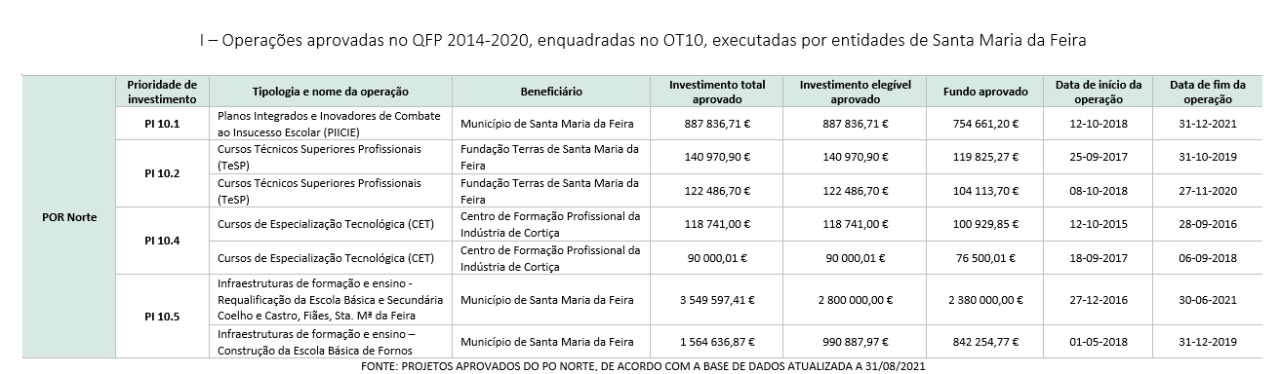
\includegraphics{C:/Users/julio/Documents/bookPoat/imagensRelatorio/img15.jpeg}

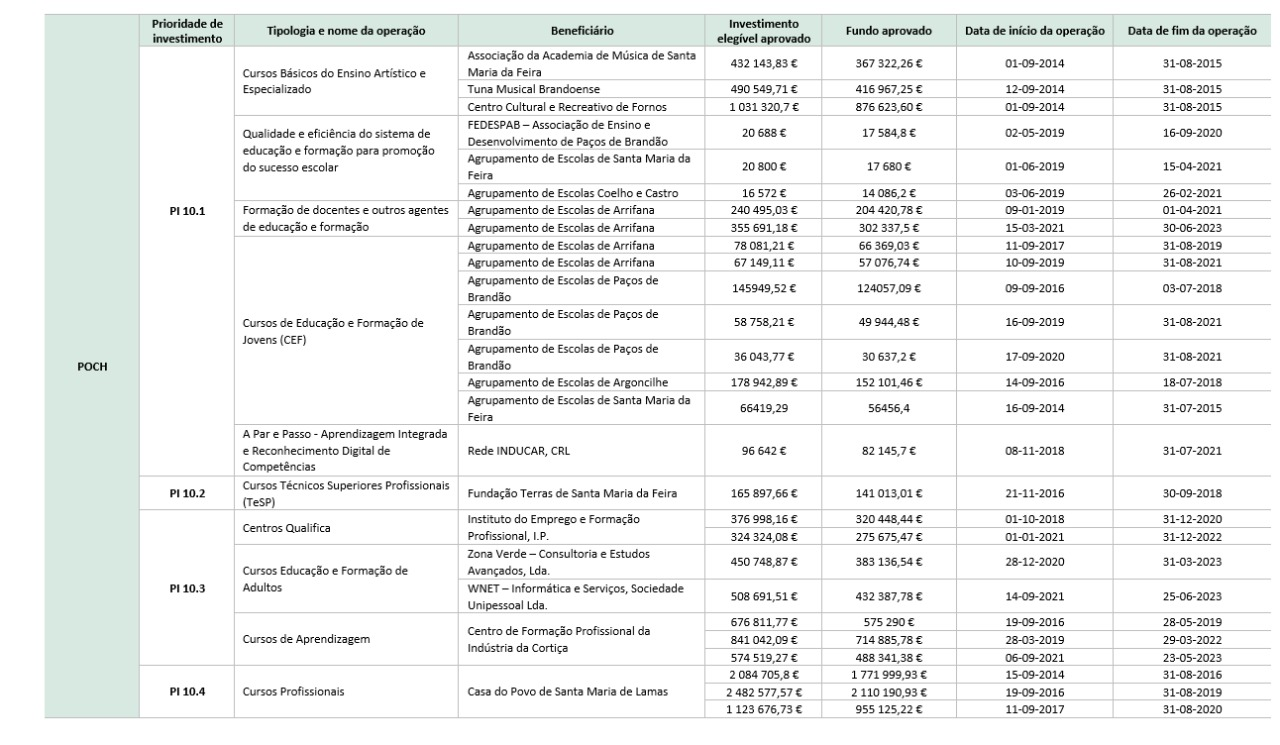
\includegraphics{C:/Users/julio/Documents/bookPoat/imagensRelatorio/img16.jpeg}

\textbf{\textbar\textbar{} -Taxas de cofinanciamento no quadro financeiro plurianual 2014-2020}

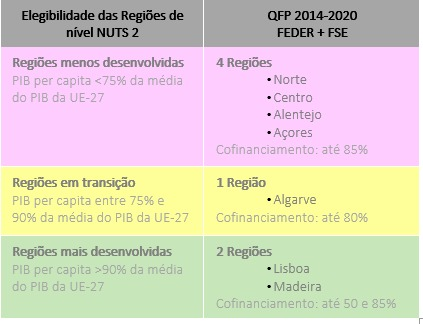
\includegraphics{C:/Users/julio/Documents/bookPoat/imagensRelatorio/img17.jpeg}

Elegibilidade das Regiões de nível NUTS 2 QFP 2014-2020
FEDER + FSE
Regiões menos desenvolvidas
PIB per capita \textless75\% da média do PIB da UE-27 4 Regiões
• Norte
• Centro
• Alentejo
• Açores
Cofinanciamento: até 85\%
Regiões em transição
PIB per capita entre 75\% e 90\% da média do PIB da UE-27 1 Região
• Algarve
Cofinanciamento: até 80\%
Regiões mais desenvolvidas
PIB per capita \textgreater90\% da média do PIB da UE-27 2 Regiões
• Lisboa
• Madeira
Cofinanciamento: até 50 e 85\%
No que concerne não o número de operações, mas o volume de cofinanciamento aprovado para os PIICIE, em cada região, importa considerar as diferentes taxas de cofinanciamento regionais, por via dos níveis de desenvolvimento, traduzidos através do PIB per capita. Consideradas menos desenvolvidas, as regiões do Norte, Centro, Alentejo e Açores podem ter um cofinanciamento europeu até 85\%, enquanto o Algarve (região em transição) tem cofinanciamento até 80\% e Lisboa, por ser mais desenvolvida, tem cofinanciamentos até 50\%. Por fim, a região da Madeira, ainda que o seu PIB per capita a torne uma região mais desenvolvida, é simultaneamente uma região ultraperiférica, pelo que as suas taxas de cofinanciamento podem também alcançar 85\%.

\textbf{\textbar\textbar\textbar{} -- Indicadores específicos das ações}

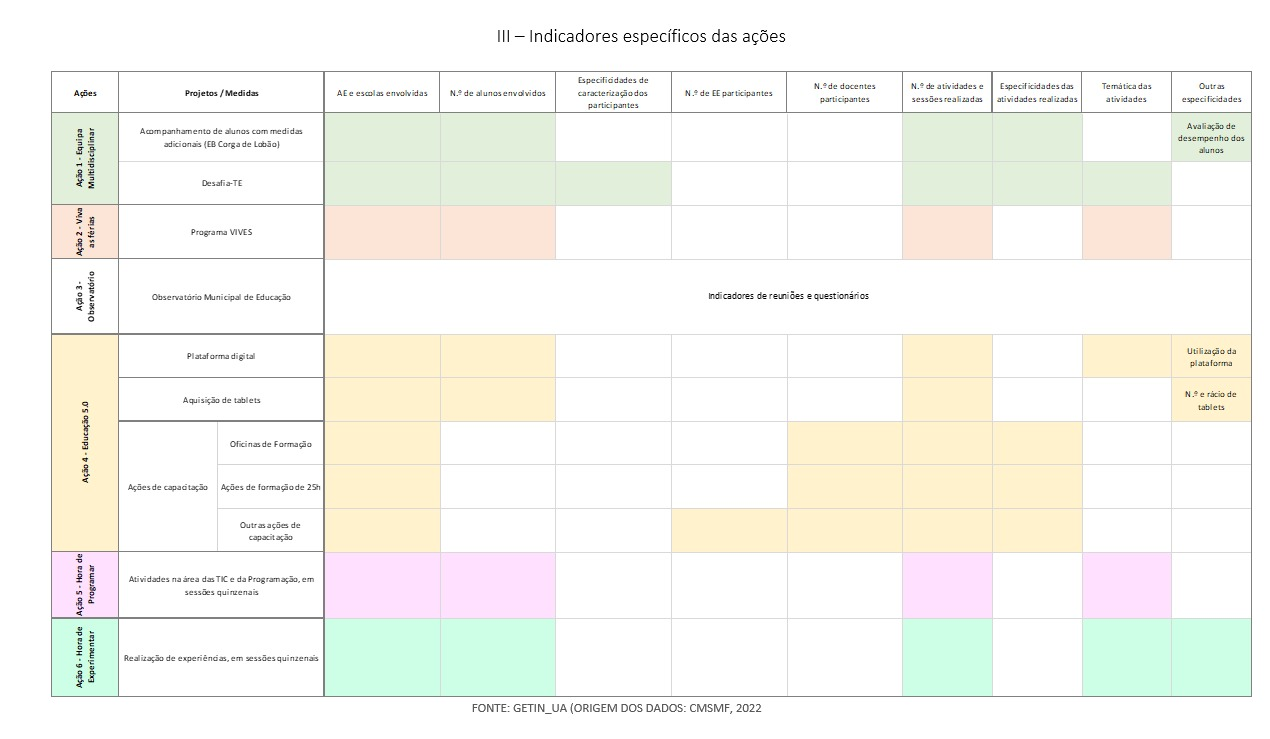
\includegraphics{C:/Users/julio/Documents/bookPoat/imagensRelatorio/img18.jpeg}

\textbf{\textbar\textbar\textbar\textbar{} --Outputs complementares produzidos ao longo do período de execução do projeto}

\textbf{Apresentações em conferências e congressos científicos:}
• `Os fundos comunitários e a política educativa em Portugal no quadro 2014-2020: Mapeamento das operações PIICIE', no 28.º Congresso da Associação Portuguesa de Desenvolvimento Regional (APDR) -- Green and inclusive transitions in Southern European regions: What can we do better, realizado em Vila Real, entre 16 e 17 de setembro de 2021
• `A monitorização de políticas educativas locais: o caso de um município da Área Metropolitana do Porto', no IV Colóquio Internacional de Ciências Sociais da Educação, realizado em Braga, entre 12 e 14 de maio de 2022
• `Desafios do processo de avaliação ex-post de uma política educativa cofinanciada', no IV Colóquio Internacional de Ciências Sociais da Educação, realizado em Braga, entre 12 e 14 de maio de 2022
• `Distribuição dos fundos estruturais associados à Educação no quadro 2014-2020 em Portugal: padrões e singularidades regionais das políticas educativas', no 29.º Congresso da APDR - Islands and peripheral territories: challenges in a moving geography and changing climate patterns, entre 29 e 30 de junho de 2022
• `Oportunidades na redefinição de princípios para a programação de equipamentos educativos', no 29.º Congresso da APDR - Islands and peripheral territories: challenges in a moving geography and changing climate patterns, entre 29 e 30 de junho de 2022

\textbf{Publicações de artigos científicos:}
• Artigo submetido, a aguardar revisão: `Os fundos comunitários e a política educativa em Portugal no quadro 2014-2020: Mapeamento das operações PIICIE'
• `Desafios do processo de avaliação ex-post de uma política educativa cofinanciada' nos proceedings do IV Colóquio Internacional de Ciências Sociais da Educação

\textbf{Trabalhos académicos, no âmbito de unidades curriculares do Mestrado de Ciências de Dados para Ciências Sociais (Universidade de Aveiro):}
• `Painéis de informação sobre territórios educativos' (Unidade Curricular: Seminário)
• `Taxas de retenção na AMP' (título provisório; Unidade Curricular: Econometria Espacial e Temporal)

  \bibliography{book.bib,packages.bib}

\end{document}
